\documentclass[a4paper, twoside]{report}

%% Language and font encodings
\usepackage[english]{babel}
\usepackage[utf8x]{inputenc}
\usepackage[T1]{fontenc}

%% Sets page size and margins
\usepackage[a4paper,top=2.5cm,bottom=2.5cm,left=3cm,right=3cm,marginparwidth=1.75cm]{geometry}

%% Useful packages
\usepackage{amsmath}
\usepackage{amssymb}
\usepackage{bm}
\usepackage{mathrsfs}
\usepackage{graphicx}
\usepackage{booktabs}
\usepackage{multirow}
\usepackage[colorinlistoftodos]{todonotes}
\usepackage{parskip}
\usepackage{caption}
\usepackage[colorlinks=true, allcolors=blue]{hyperref}
\usepackage[nameinlink,capitalise]{cleveref}
\usepackage{bbm}
\usepackage{amsthm}

\theoremstyle{definition}
\newtheorem{definition}{Definition}[chapter]


\title{Data Poisoning Attacks against Adaptive (Continual) Learning}
\author{Dillan Scott}

\begin{document}
\input{title/title.tex}

\begin{abstract}
Adaptive intrusion-detection systems pair a drift detector with a base learner that retrains whenever the detector registers a new concept. The Contrastive NCM detector of Kuppa and Le-Khac couples a contrastive autoencoder to a nearest-class-mean classifier and is reported to be adversarially robust --- but only as a stand-alone detector. We evaluate it as it would be deployed: coupled to a downstream classifier whose retraining it triggers, on the Engelen-corrected CICIDS2017 stream. We find that the coupling, not the representation, is the exploitable surface, and that the adversary's leverage is over the system's adaptation rather than its decision boundary. An aimed feature-space mean-shift forces a spurious concept-discovery event both white-box and grey-box --- retaining roughly $70\%$ of its effect against a detector trained on disjoint data --- because the batch-mean statistic the detector adopts for stability transfers far better than the per-sample detection it is built on. A firing gate added to stop premature retraining is double-edged: an ablation proves that any constraint on the retraining buffer's makeup that resists this forcing simultaneously lets an attacker suppress adaptation by dilution, starving the system of the updates it needs. A base learner retrained correctly resists low-rate poisoning of its decision boundary, yet the detector silently fails to discover one of two novel attack classes because it embeds too close to a known one. Coupling a robust detector to a base learner does not inherit its robustness; it creates new timing- and composition-based attack surfaces that a detector-only evaluation cannot see.
\end{abstract}

\tableofcontents
\listoffigures
\listoftables
\listoftodos

\chapter{Introduction}
\label{ch:introduction}

\section{Context and Motivations}
It is becoming increasingly necessary for machine learning systems to operate in dynamic environments where data arrives as a stream with no guarantees about its underlying distribution. Examples include fraud detection, network intrusion detection, and content moderation, where new observations are generated sequentially, and historical data may eventually become outdated.

Learning under these conditions is referred to as adaptive or continual learning. In contrast to traditional batch learning, where models are static post-deployment, adaptive models are repeatedly updated. The motivation for these online updates is not only to handle the volume or velocity of streaming data, but also to account for concept drift - changes in the joint distribution of inputs and outputs over time. The performance of a static model, which is accurate on current data, may degrade as the environment changes. Consequently, mechanisms known as drift detectors are used to monitor incoming data streams and signal the need for model updates when necessary.

While drift detection has been extensively studied in non-adversarial settings~\cite{Gao_2007, Gama_2014, Barros_2018}, critical security concerns arise when operating in environments where strategic or malicious actors may influence data streams. In domains such as fraud detection and cybersecurity, adversaries may deliberately manipulate data to evade detection, degrade model performance, or force harmful model adaptations. Unlike poisoning attacks against fixed models, adversarial attacks against adaptive systems can aim to exploit the update mechanism - using it as a vector to inject malicious concepts, suppress valid adaptations, or corrupt the detector's learned representation.

In response to this threat, recent research has proposed adversarially robust drift detectors. The contrastive autoencoder and Nearest Class Mean (NCM) detector of Kuppa and Le-Khac~\cite{Kuppa_2022}, the target system of this work, uses a contrastive loss to map inputs into a latent space where same-class samples cluster tightly, classifies incoming samples by their distance to learned class prototypes using a combined Euclidean and Riemannian metric designed to reject adversarial subspaces, and grows the prototype set automatically when the accumulated displacement of drifted embeddings crosses a threshold. Another approach by Korycki and Krawczyk~\cite{Korycki_2022} pursues similar goals through reconstruction-error monitoring with an energy-based model, specifically a Robust Restricted Boltzmann Machine. Both have demonstrated robustness against certain poisoning strategies.

However, both works share a fundamental limitation when viewed from the perspective of a fully coupled adaptive learning pipeline. Kuppa and Le-Khac~\cite{Kuppa_2022} evaluate their detector in isolation: their experiments measure the detector's ability to correctly classify incoming samples as drifted or not, reporting precision, recall and F1 against held-out drifted classes. No downstream base learner is used, meaning their robustness claims speak only to the detector's own classification performance and say nothing about whether those properties extend to protecting a separate model that depends on the detector to govern its adaptation. Korycki and Krawczyk~\cite{Korycki_2022} do include a base learner, but they choose a model that updates continuously, instance by instance, regardless of drift signals; meaning the detector is advisory rather than controlling.

This discrepancy is significant... Understanding these limitations...\todo[color=red]{Finish this paragraph}

\section{Scope}
\label{sec:scope}
This thesis examines adversarial attacks against an adaptive learning pipeline consisting of a static MLP classifier coupled with the contrastive auto-encoder and Nearest Class Mean detector~\cite{Kuppa_2022}. The work is centred on understanding whether this state-of-the-art robust detector is sufficient to protect a trigger-dependent base learner when the two components are deployed together as a coupled system.

This work takes an adversarial perspective, proposing attacks against the coupled system, covering those on each element both individually and simultaneously. A representative subset of these attacks is then implemented and evaluated, selected to span the primary ways in which an adversary could exploit the system's coupling.

% Rather than introducing a new drift detection algorithm, this thesis adopts an adversarial perspective. It proposes a novel feedback-guided attack strategy that operates under a closed-loop threat model, in which the attacker adapts their behaviour based on downstream observable feedback. This attack is used as a systematic stress test for existing adversarially robust drift detectors, allowing the evaluation of their effectiveness under stronger and more realistic assumptions about the attacker's behaviour.

The aim is not to refute the robustness claims of Kuppa and Le-Khac~\cite{Kuppa_2022} but to test whether those claims extend to the protection of a downstream base learner in a realistic adaptive learning architecture. By doing so, the thesis seeks to clarify the practical security guarantees offered by the detector and identify the conditions under which the coupled system remains vulnerable.

\section{Objectives}
The primary objective of this research is to determine whether the robustness of the contrastive auto-encoder and NCM detector is sufficient to protect a static, trigger-dependent base learner from corruption when the two components are deployed as a coupled adaptive learning system.

First, it formalises a taxonomy of attacks against the coupled system and identifies the structural properties of trigger-dependent architectures that create attack surfaces absent from prior evaluations. Second, it implements and experimentally analyses whether each attack can successfully harm the base learner's predictive capabilities.\todo[color=red]{More here?}

% The primary objective of this research is to critically evaluate the resilience of concept drift detection mechanisms against adaptive adversaries. First, this thesis will formalise a taxonomy of threat models, explicitly distinguishing between open-loop and closed-loop, to define how attackers exploit system outputs. Building on this framework, the thesis aims to propose a novel feedback-guided attack strategy designed to induce semantic drift while avoiding detection thresholds.

% Subsequently, this work will experimentally analyse the vulnerability of existing adversarially robust drift detectors to determine if they can be evaded by such adaptive strategies. Finally, the thesis seeks to characterise the boundaries of effective detection, identifying the fundamental trade-offs between sensitivity to natural drift and robustness against adversarial manipulation.


\section{Research Questions}
\label{sec:research questions}
To meet the objective described in the previous section, this thesis addresses the following questions:
\begin{enumerate}
    \item How can the capabilities and knowledge of an adversary targeting a coupled adaptive learning system be formally defined, and what attack surfaces are introduced by trigger-dependent base learner architectures that are absent when the base learner updates continuously?

    \item Can an adversary successfully corrupt the predictive accuracy of a static base learner by exploiting the retraining mechanism of a system equipped with the contrastive auto-encoder and NCM detector, despite its robustness properties?
    
    \item Can an adversary corrupt the detector's learned representation sufficiently to manipulate the adaptation of the base learner — either by forcing false retraining events or by suppressing valid ones?

    \item What ongoing poisoning budget, in instance count and perturbation magnitude, is required to maintain these adversarial effects against a detector that continuously updates its representation of the data distribution?

    \item What is the trade-off between the detector's robustness to adversarial poisoning and its sensitivity to genuine concept drift, and how does this manifest in a trigger-dependent coupled architecture?
\end{enumerate}

\section{Thesis Structure}
The remainder of this thesis is organised as follows: 
\begin{itemize}
    \item \cref{ch:background} reviews the background literature on continual learning and adversarial attacks. 
    
    \item \cref{ch:target_system_threat_model} formalises the target system and establishes the threat model, defining the adversary's objectives, knowledge, and capabilities.
    
    \item \cref{ch:attack_taxonomy_objectives} presents a taxonomy of attacks against the coupled system and introduces the idea of maintenance cost. 
    
    % \item \cref{ch:project} lays out what needs to be done to complete the project and an expected timetable.
    
    % \item \cref{ch:evaluation} explains what the evaluation process will be and what is necessary to constitute success.
    
    % \item \cref{ch:ethics} provides a discussion of wider ethical, legal, professional and societal issues surrounding this project and the accompanying research.
\end{itemize}
\chapter{Background}
\label{ch:background}

This chapter establishes the theoretical foundations and reviews the relevant literature to contextualise the later contents of this thesis. It begins by formally defining concept drift and outlining its taxonomy based on probabilistic decomposition and temporal characteristics. Subsequently, the general architecture of drift detection systems is analysed, alongside a review of some existing concept drift detectors and their inherent limitations. The chapter then moves on to consider a security perspective, introducing the notion of adversarial concept drift, where distributional shifts are manipulated by potentially malicious actors. Before turning to defences, it introduces the foundations of class-incremental learning and exemplar-based memory, which underpin how adaptive learners update without forgetting. Finally, the chapter concludes by discussing the already existing robust solutions, which have been proposed to mitigate these challenges.

\section{Concept Drift}
Concept drift generally refers to changes in the statistical relationship between input features and target labels, characterised as a change in the true joint distribution $p(X, y)$~\cite{Gao_2007}. Formally, concept drift between time points $t_0$ and $t_1$ is said to occur when
\begin{equation}
    p_{t_0}(X, y) \neq p_{t_1}(X, y),
\end{equation}
where $p_{t_0}$ and $p_{t_1}$ denote the joint distributions of the input variables $X$ and target variable $y$ at times $t_0$ and $t_1$, respectively~\cite{Gama_2014}.

\subsection{Taxonomy of Drift}
\subsubsection{Probabilistic Nature}
The joint probability can be given by the decomposition 
\begin{equation}
    p(X, y) = p(y \mid X)p(X)
\end{equation}
where $p(y \mid X)$ is the conditional distribution of the target given the input features and $p(X)$ is the probability distribution of the input features. Based on this, the literature~\cite{Gao_2007, Gama_2014, Korycki_2022} distinguishes between two forms of concept drift:

\begin{enumerate}
    \item \textit{Real drift}: When $p(y \mid X)$ changes without a change in $p(X)$ (Conditional Change) or with it (Dual Change). This is the more critical form of drift, as it directly affects decision rules or classification boundaries, making model adaptation necessary.
    
    \item \textit{Virtual drift (feature change)}: When $p(X)$ changes without affecting $p(y \mid X)$. While this may appear less important than real drift because the decision function is left unchanged, it cannot be ignored. In particular, changes in $p(X)$ may trigger adaptation or forgetting mechanisms, potentially leading to unnecessary or even harmful model updates.
\end{enumerate}

\subsubsection{Temporal Characteristics}
In addition to the above types, based on probabilities, concept drift can be categorised based on how the change occurs over time. Namely, four common patterns are shown in~\cref{fig:drift types}~\cite{Lu_2018}.

\begin{enumerate}
    \item \textit{Sudden/abrupt drift} is when the instance distribution or concept changes within a very short time frame. The previous concept immediately becomes invalid, and the learner must adapt quickly to maintain performance~\cite{Korycki_2022}.
    
    \item \textit{Gradual drift} is where instances from the old and new concepts coexist for a period, with old appearing with decreasing frequency~\cite{Korycki_2022}.
    
    \item \textit{Incremental drift} is when there is a smooth and continuous progression from one concept to another through a series of intermediate concepts~\cite{Gama_2014, Korycki_2022}.
    
    \item \textit{Reoccurring concepts} refers to when previously seen concepts reappear after some time, such as in seasonal or cyclical patterns~\cite{Gama_2014}. They may reappear either suddenly or incrementally~\cite{Guzy_2020}.
\end{enumerate}

\begin{figure}[h]
    \centering
    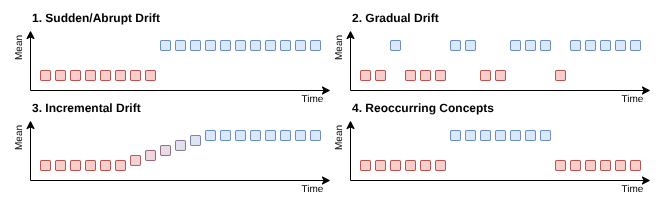
\includegraphics[width=\linewidth]{background/drift types.drawio.png}
    \caption{Examples of concept drift types based on temporal patterns}
    \label{fig:drift types}
\end{figure}


\section{Concept Drift Detection}
\label{sec:drift_detection}
In data stream learning, concept drift is typically addressed by augmenting the predictive model (the base learner) with a drift detection mechanism. In general, drift detectors attempt to identify changes in the data distribution by analysing the base learner's behaviour~\cite{Barros_2018}. Rather than continuously retraining the learner, drift detectors act as a supervisory mechanism, triggering an adaptation process, such as model retraining, parameter update, or selective forgetting of historical data.

\subsection{General Architecture of Drift Detection Systems}
\label{sec:drift detection architecture}
Although they are algorithmically diverse, most concept drift detection systems follow a common architectural pattern. This architecture can be decomposed into four conceptual components:

\begin{enumerate}
    \item \textit{Observation source}: The detector monitors a stream of signals derived either from the data itself or from the performance of a base learner. Common sources include error rates, loss values, feature statistics, or latent representations.
    
    \item \textit{Summary mechanism}: Observations are aggregated over time using sliding windows, cumulative statistics, or incremental estimators. This step compresses the raw stream into a tractable representation that reflects the system behaviour of a given period.
    
    \item \textit{Change test}: A statistical test, threshold comparison, or learned decision rule evaluates whether the observed summary deviates significantly from a reference/historical summary. This comparison may rely on bounds derived from concentration inequalities, hypothesis tests, or reconstruction error metrics.
    
    \item \textit{Decision and response}: Upon detecting significant deviation, the detector emits a signal (sometimes distinguishing between a warning and confirmed drift) which triggers downstream actions such as retraining, window resetting, or model replacement.
\end{enumerate}

This modular structure highlights an important property of drift detectors: they act as \emph{control mechanisms} governing when and how adaptive learning occurs. As such, their behaviour has long-term consequences for system performance, stability, and robustness.

\subsection{Drift Detection Algorithms}
While the general architecture remains consistent, specific implementations differ in their observation sources and statistical tests. The literature typically categorises these methods into error rate-based and data distribution-based approaches~\cite{Lu_2018}.

\subsubsection{Error Rate-Based Detectors}
These methods monitor the online performance of the base learner (e.g. classification accuracy). They function based on the assumption that a statistically significant increase or decrease in model performance implies a change in the underlying data distribution~\cite{Lu_2018}. Drift detectors in this category include:

\begin{itemize}
    \item \textit{Drift Detection Method (DDM)}~\cite{Gama_2004}: This method models the number of errors as a random variable from a Binomial distribution. It tracks the online error rate $p_t$ and its standard deviation $s_t = \sqrt{p_t(1-p_t)/t}$ at time $t$. The algorithm maintains the minimum values observed so far, $p_{min}$ and $s_{min}$, updating them whenever $p_t + s_t < p_{min} + s_{min}$. A warning level is triggered if: 
    \begin{equation} \label{eq:DDM warning}
        p_t + s_t \geq p_{min} + 2s_{min},
    \end{equation}
    at which point incoming examples are buffered while using the old learner for predictions. If the error rate continues to rise and drift is confirmed via the condition: 
    \begin{equation} \label{eq:DDM confirmation}
        p_t + s_t \geq p_{min} + 3s_{min},
    \end{equation}
    a new learner is induced using the buffered examples, and the old learner is discarded.
    % DDM is effective for detecting abrupt drift but can be less sensitive to gradual changes or noisy data streams.

    \item \textit{ADaptive WINdowing (ADWIN)}~\cite{Bifet_2007}: This method uses a sliding window $W$ that dynamically adjusts its size, based on the rate of change in the data stream. It operates by examining all possible cuts of the current window into two sub-windows, $W_{0}$ and $W_{1}$, representing historical and newer data, respectively. Drift is detected if the absolute difference between the averages of these sub-windows is statistically significant:
    \begin{equation} \label{eq:ADWIN threshold}
        |\hat{\mu}_{W_0} - \hat{\mu}_{W_1}| \geq \epsilon_{cut}
    \end{equation}
    where $\epsilon_{cut}$ is an adaptive threshold (determined using Hoeffding bounds and a confidence interval $\delta$). When this threshold is reached, the historical data ($W_{0}$) is discarded as the two sub-windows are seen to have come from different data distributions. The author's also proved that the false positive and false negative rates are bounded by $\delta$.
\end{itemize}

\subsubsection{Data Distribution-Based Detectors}
In contrast, these methods monitor the statistical properties of the input features ($P(X)$), independent of the base learner's behaviour and error rate. They rely on the assumption that drift can be signalled by a statistically significant deviation in the distribution of new data when compared to a historical reference window~\cite{Lu_2018}. Because they analyse the input data itself, these methods can detect virtual drift that does not immediately alter the decision boundary and can also function when ground truth labels are unavailable. Examples of data distribution-based detectors include:

\begin{itemize}
    \item \textit{Statistical Change Detection for multidimensional data (SCD)}~\cite{Song_2007}: This detector addresses the challenge of multidimensional distribution change by employing a non-parametric statistical test known as the Density Test. The baseline/historical window $S$ is partitioned into two halves: $S_1$ for modelling and $S_2$ for testing. It utilises a Kernel Density Estimator (KDE) on $S_1$, to get the density function $\mathscr{K}_{S_1}$. The test statistic $\delta$ is then defined using the difference in log-probability density of $\mathscr{K}_{S_1}$ at $S'$ and at $S_2$. Specifically:
    \begin{equation}
        \delta = LLH(\mathscr{K}_{S_1}, S') - \frac{|S'|}{|S_2|} \times LLH(\mathscr{K}_{S_1}, S_2)
    \end{equation}
    where $LLH$ is the log-likelihood. Drift is confirmed if $\delta$ falls below a critical value $C_{max}$ (algorithmically derived from a user-defined significance level $p$).

    \item \textit{Principal Component Analysis-Based Change Detection (PCA-CD)}~\cite{Qahtan_2015}: This method works on multidimensional data streams by projecting the data onto lower-dimensional spaces using PCA. It extracts the top $k$ principal components that explain a substantial portion of the variance from the historical window and then monitors new data projected onto these components as separate univariate streams. Similarly to SCD, the density of these projections is estimated using KDE, for example. A divergence metric, such as the intersection area under the curves of the reference ($\hat{f}$) and test ($\hat{g}$) distributions:
    \begin{equation}
        D_{A}\left(\hat{g}\,||\,\hat{f}\right) = 1 - \int_{x} \min\left(\hat{f}(x), \hat{g}(x)\right) dx
    \end{equation}
    is calculated for each of the $k$ components. Then the final change score is taken as the maximum of these. To detect drift, the method applies the Page-Hinkley (PH) test with a dynamic threshold to the aggregate score, triggering an alarm when the cumulative deviation from the historical mean exceeds a given limit.
\end{itemize}

\subsection{Limitations and Weaknesses}
While the drift detectors described above do provide robust mechanisms for adaptation, they are subject to inherent limitations and trade-offs between sensitivity (minimising false negatives) and specificity (minimising false positives). Rather than arising from flawed algorithms, many of these weaknesses are due to the statistical assumptions made by classical drift detection; most notably, finite-sample estimation, approximate stationarity within windows, and the use of fixed confidence bounds to identify change.

These limitations can be mapped onto the general architecture of drift detectors introduced earlier in~\cref{sec:drift detection architecture}. Choices made at the level of the observation source (e.g. error rates or feature statistics), the summary mechanism (e.g. windowing or cumulative statistics), and the change test (e.g. hypothesis tests or thresholds) impose constraints on what types of drift can be reliably identified and how quickly.

\subsubsection{Sensitivity to Gradual Drift}
A limitation of some error-based detectors, such as DDM, is the reduced ability to distinguish between stationary noise and gradual concept drift. In the presence of abrupt drift, the error rate typically exhibits a sharp increase, triggering the detector's thresholds (defined for DDM in~\cref{eq:DDM warning} and~\cref{eq:DDM confirmation}). However, during a gradual drift, the error rate may increase too slowly to violate the statistical bounds.

Under such conditions, the detector may update its internal reference statistics ($p_{min}$ and $s_{min}$ in the case of DDM), effectively incorporating the drifted distribution into its baseline instead of identifying it. While adaptive windowing approaches, such as ADWIN, mitigate this by dynamically adjusting the window size, they are still bounded by the resolution of their sliding window. Drift, which remains below the statistical bound (defined for ADWIN as $\epsilon_{cut}$ in~\cref{eq:ADWIN threshold}), will remain undetected until enough samples accumulate to reach statistical significance.

Fundamentally, this limitation highlights the difficulty in distinguishing between slow drift and stationary noise under bounded confidence levels, without making additional assumptions about the drift process. Any attempt to increase sensitivity by lowering detection thresholds inevitably raises the false positive rate, highlighting a trade-off key to all hypothesis test-based or threshold-based drift detectors.

\subsubsection{Verification Latency and Label Availability}
Error-based detectors suffer from a critical dependency on ground truth availability. They assume that labels are available immediately or with minimal delay after the prediction is made, to compute prediction errors and monitor performance degradation. In many real-world streaming applications, such as credit fraud detection or loan forecasting, the true label may arrive with significant delay (verification latency) or may never arrive at all. 

During periods of high verification latency, the detector effectively cannot observe its primary signal, leaving the system blind to changes in performance. If drift occurs during such a period, the system will continue to trust an outdated model, accumulating loss until detection becomes possible.

\subsubsection{Virtual Drift and False Positives}
Distribution-based detectors address the problem with label dependency by monitoring the input feature distribution $P(X)$ rather than model error. While this enables detection in settings with delayed or missing labels, it introduces a different weakness related to virtual drift. A statistically significant change in $P(X)$ does not always imply a change in the conditional distribution $P(y \mid X)$. It therefore does not guarantee that the predictive decision boundary has changed.

Consequently, distribution-based detectors may generate false positives, triggering model retraining or data forgetting even when performance remains stable (there is no real drift). Such unnecessary adaptation can be computationally expensive and may temporarily degrade performance.

\subsubsection{Dimensionality and Feature Relevance}
In high-dimensional settings, distribution-based detectors rely on density estimation or projection techniques that are sensitive to the curse of dimensionality. As the number of dimensions increases, data sparsity reduces the reliability of density estimates, while dimensionality reduction risks discarding directions along which drift is relevant. Moreover, distribution-based detectors typically treat all features with equal importance, meaning they are susceptible to changes in weakly relevant features that may not materially affect model performance.


\section{Adversarial Concept Drift}
Classical concept drift assumes that changes in the data distribution arise from natural, exogenous factors such as evolving user behaviour, seasonality, or changes in the underlying environment. In contrast, adversarial drift assumes that there is a purposeful and potentially malicious actor attempting to manipulate our adaptive learning system~\cite{Korycki_2022}. The potential goals they may have will be discussed in the next section. 

In such settings, the drift process is no longer passive. Instead, the data stream itself becomes an attack surface, and the drift detector becomes a target. Adversarial drift extends traditional data poisoning attacks by exploiting temporal dynamics and specific detector behaviours. Rather than corrupting a static training set, the adversary seeks to control when adaptation is triggered, what data is included during retraining, and which information is forgotten. This introduces a new class of threats that cannot be fully explained by classical adversarial learning models alone~\cite{Kloft_2010}.

\subsection{Adversarial Objectives}
An adversary interacting with an adaptive learning system may pursue several objectives, which are not mutually exclusive.

A primary objective could be \emph{performance degradation}, where the adversary seeks to reduce the predictive accuracy or increase the loss of a system~\cite{Sethi_2018}. Unlike poisoning attacks, adversarial drift may be gradual, ensuring that degradation accumulates slowly while remaining below detection thresholds.

This could be seen as a potential secondary objective: \emph{evasion of detection}. Here, the adversary aims to avoid the activation of the drift detector while pursuing their primary objective. This could involve crafting inputs that move the decision boundary while preserving the statistics monitored, hence exploiting the blind spots of classical detectors.

Alternatively, an adversary may attempt \emph{forced adaptation}, deliberately triggering false drift alarms to cause unnecessary retraining or forgetting. Such behaviour can destabilise the learning process, increase computational costs, or induce catastrophic forgetting of valid historical concepts~\cite{Korycki_2022}. Conversely, an adversary could seek to \emph{block adaptation}, injecting contradictory data points during a period of valid concept drift, in an attempt to nullify the adaptation process~\cite{Korycki_2022}.

Finally, adversaries may seek \emph{control over the learned concept}, gradually forcing the system to learn a decision boundary favourable to the attacker’s goals. In this case, the detector is actively exploited as a mechanism for injecting the poisoned instances during adaptation cycles.

\subsection{Instance-Based Poisoning}
Instance-based poisoning attacks are those in which an adversary injects or modifies individual data points in the stream to influence the base learner or drift detector. These attacks are powerful because the poisoned instances can be distributed over time, allowing adversaries to exploit both the learner’s update behaviours and the detector’s temporal assumptions. For example, poisoned samples may be injected intermittently or gradually, ensuring that individual instances appear benign while the cumulative effect leads to performance degradation or detector manipulation.

From a drift detection perspective, instance-based poisoning can be used to:
\begin{itemize}
    \item \textit{Bias summary statistics}: By subtly increasing error rates or similar statistics within certain bounds, the adversary can influence the detector's inner mechanisms.
    \item \textit{Trigger false alarms}: Bursts of or extreme poisoned instances may surpass thresholds, triggering unnecessary adaptation or window resets.
    \item \textit{Suppress true drift detection}: Conversely, carefully engineered samples can stabilise monitored statistics during periods of genuine drift, delaying or preventing detection~\cite{Korycki_2022}.
\end{itemize}

Crucially, even small, strategically placed perturbations can be sufficient to accumulate and have the desired effect, particularly against detectors based on hypothesis testing or confidence bounds. This makes instance-based poisoning difficult to distinguish from natural noise or gradual drift, especially in high-variance data streams.

% While many drift detectors incorporate safeguards such as conservative thresholds, ensemble monitoring, or robust statistics, these defences are designed under the assumption of stochastic rather than adversarial data generation. As a result, they may remain vulnerable to coordinated instance-level attacks that exploit their reliance on finite-sample estimates and bounded confidence levels.

\subsection{Concept-Based Poisoning}
Concept-based attacks function at a higher level of abstraction than instance-based attacks. Rather than focusing on individual samples, the adversary aims to directly mimic a shift in the data-generating process to falsify genuine concept drift. The adversary engineers the drift trajectory to achieve a desired outcome, such as the misclassification of specific regions of the input space or the biased treatment of certain inputs.

By anticipating how the detector responds to changes in monitored statistics, the adversary can:
\begin{itemize}
    \item \textit{False adaptation}: Triggering adaptation where the system interprets the adversarial concept as a genuine distributional change~\cite{Korycki_2022}.
    \item \textit{Exploit forgetting mechanisms}: Causing the system to discard historically valid or important data.
    \item \textit{Suppressed adaptation}: Balancing genuine concept drift with a conflicting distribution, preventing the detector from reaching its change threshold or negatively impacting the adaptation process.
\end{itemize}

% Such attacks are particularly effective against detectors designed to respond to gradual or incremental drift. By aligning the induced change with expected temporal patterns, the adversary can ensure that adaptation mechanisms are triggered naturally, causing the learner to internalise a corrupted concept as if it were benign~\cite{Koh_2021}.


\section{Class-Incremental Learning and Exemplar Memory}
\label{sec:exemplar memory}
The drift detectors described so far are concerned with deciding when to adapt. Equally important is how a model is updated once said adaptation is triggered. When a learner is only retrained on newly arrived data, it can overwrite previously learned knowledge, a phenomenon known as catastrophic forgetting~\cite{French_1999}. This is especially problematic in streaming settings where reoccurring concepts are common and may reappear after the model has specialised to more recent traffic.

A common countermeasure is rehearsal (or replay), where a small memory of representative past examples, called exemplars, is retained and used alongside new data during each update~\cite{Robins_1995}. Given a finite memory budget, an important question is which examples to keep so the retained subset remains faithful to the data it summarises.

A widely adopted solution is the iCaRL (Incremental Classifier and Representation Learning) mechanism introduced by Rebuffi et al.~\cite{Rebuffi_2017}, which classifies using a nearest-mean-of-exemplars rule. Given a class with feature embedding $\phi(\cdot)$ and true mean
\begin{equation}
    \mu = \frac{1}{n}\sum_{x} \phi(x),
\end{equation}
herding greedily builds an ordered exemplar set $\{p_1, \dots, p_m\}$ of target size $m$, selecting the $k^{\text{th}}$ exemplar as the sample that brings the running exemplar mean closest to $\mu$:
\begin{equation} \label{eq:herding}
    p_k = \arg\min_{x} \left\| \mu - \frac{1}{k}\left( \phi(x) + \sum_{j=1}^{k-1} \phi(p_j) \right) \right\|.
\end{equation}
Because each successive exemplar maximally reduces the difference between the stored mean and the true class mean, any prefix of the resulting set remains representative of the class centroid, and the budget $m$ can be adjusted without re-selecting from scratch.

This property is particularly valuable for nearest-mean classifiers operating under bounded memory. Since the class prototype is computed from the stored exemplars rather than the full data history, a herded memory preserves the representation of that prototype while bounding both storage and retraining cost. This makes it a natural memory-management policy for an NCM-based drift detector that must register newly discovered concepts and retain a limited, representative sample of each for future retraining, a point we return to when describing the drift detector adopted in this thesis (\cref{sec:contrastive_ncm}).


\section{Adversarially Robust Solutions}
\label{sec:robust solutions}
To address the vulnerabilities of traditional detectors, recent research proposes methods explicitly designed to withstand adversarial manipulation. These solutions employ techniques like contrastive embedding and generative modelling to differentiate between natural and adversarial distributional shifts.

\subsection{Robust Restricted Boltzmann Machine for Drift Detection}
\label{sec:rrbm-dd}
Korycki and Krawczyk~\cite{Korycki_2022} introduce the Robust Restricted Boltzmann Machine for Drift Detection (RRBM-DD), a generative neural network that detects drift by monitoring the reconstruction error of incoming samples against a learned model of the past data distribution. That is, the RRBM encodes the recent distribution directly in its weights and the detector treats any sample that the model fails to reconstruct accurately as evidence of distributional change. The architecture also incorporates two distinct mechanisms designed to remain robust when the incoming stream is adversarially manipulated rather than naturally drifting.

To counter instance-based poisoning, the model is trained with a robust gradient descent procedure using M-estimators that softly truncate the influence of samples whose loss exceeds a learned tolerance. To counter concept-based poisoning, the model's energy function is augmented with a gating mechanism over the hidden layer and a Gaussian noise model over the visible layer. The gating allows individual hidden units to be deactivated when their contribution is dominated by an adversarial cluster, and the noise model damps reconstruction-error spikes caused by adversarial perturbations.

Korycki and Krawczyk evaluate the RRBM-DD as part of a coupled adaptive system where the downstream base learner is updated continuously. They employ an adaptive Hoeffding tree that incrementally revises its splits with each new labelled sample, independently of any drift signal. In this configuration, the detector's role is advisory: it can declare that drift has occurred, causing a full retraining, but the model still adapts continuously and so does not depend entirely on the detector to trigger updates. This contrasts with the setting examined in this thesis, in which a static base learner updates only when explicitly triggered by the detector and therefore inherits both the detector's robustness properties and its decision latency. The implications of this difference for adversarial robustness are taken up in~\cref{ch:target_system_threat_model}.

\subsection{The Contrastive NCM Detector}
\label{sec:contrastive_ncm}
% Kuppa and Le-Khac~\cite{Kuppa_2022} propose a detector that maps high-dimensional inputs to a low-dimensional latent space using a contrastive loss objective. To create tighter class clusters, which are naturally more robust to adversarial perturbations, this objective places similar samples closer together while spreading dissimilar ones apart.

Kuppa and Le-Khac~\cite{Kuppa_2022} introduce the Contrastive NCM detector, composed of three key components. A contrastive autoencoder which maps each raw input vector into a lower dimensional latent space where same-class samples cluster tightly. A Nearest Class Mean (NCM) classifier which uses a hybrid Euclidean-Riemannian distance metric to decide whether the incoming sample is consistent with one of the known classes or should be flagged as drifted. Finally, a recursive concept-discovery mechanism which accumulates drifted embeddings over time and, once a threshold is exceeded, registers a new class prototype or concept. This combination is designed to remain robust under adversarial inputs by combining the manifold-tightening effect of contrastive training with a distance metric that distinguishes adversarial samples from genuine novel ones.

\subsubsection{Contrastive Autoencoder}
The encoder $h : \mathbb{R}^d \to \mathbb{R}^r$ maps each $d$-dimensional input $x$ to a lower-dimensional latent embedding $h(x)$ (with $r < d$); we write $h_i = h(x_i)$ for the embedding of sample $x_i$. The autoencoder is trained jointly under two losses. The first is the standard mean-squared reconstruction loss
\begin{equation} \label{eq:ncm-mse}
    \mathcal{L}_{\text{MSE}} = \| g(h(x)) - x \|^2_2,
\end{equation}
where $g(\cdot)$ is the decoder. The second is a supervised contrastive term which aims to make the positive pairs attracted and the negative samples separated
\begin{equation} \label{eq:ncm-contrastive}
    \mathcal{L}_{\text{contrastive}} = - \sum_{i=1}^B \log \left[\frac{e^{s(h_i, v_k)}}{\sum_{j}^P e^{s(h_i, v_j)}}\right],
\end{equation}
where for a sample $x_i$ with embedding $h_i$ in class $k$, $v_k$ is the prototype of class $k$ in the latent space, $P$ is the number of known classes, $B$ is the batch size, and the similarity score
\begin{equation}
    s(h_i, v_j) = \frac{h_i^\top v_j}{\|h_i\| \|v_j\|} \cdot \frac{1}{\tau}
\end{equation}
is a temperature-scaled cosine similarity with temperature $\tau$. Class prototypes $v_k$ are computed as the mean embedding of samples in the batch belonging to class $k$. The combined objective $\mathcal{L} = \mathcal{L}_{\text{MSE}} + \mathcal{L}_{\text{contrastive}}$ encourages the encoder to produce a latent space that simultaneously preserves enough information to reconstruct the input (via $\mathcal{L}_{\text{MSE}}$) and clusters same-class samples tightly while pushing different-class samples apart (via $\mathcal{L}_{\text{contrastive}}$).

\subsubsection{Nearest Class Mean Classifier with Hybrid Distance}
Once the embedding network is trained, it is used to fit a Nearest Class Mean (NCM) classifier~\cite{Kuppa_2022} that decides which known class an incoming sample belongs to or whether it should be flagged as drifted. NCM is a distance-based classifier that assigns each incoming sample to the class with the closest prototype, here in latent space. Its accuracy depends critically on the choice of distance metric. For each known class $c$, the prototype is computed as the mean of the embeddings of its training samples:
\begin{equation} \label{eq:ncm-prototype}
    \bm{h}_c = \frac{1}{n_c} \sum_{i}\left[y_i=c\right] \mathbf{h}_i,
\end{equation}
where $n_c$ is the number of training samples observed for class $c$; this $\bm{h}_c$ is the full-data counterpart of the per-batch prototype $v_k$ in~\cref{eq:ncm-contrastive}, both being the latent-space centroid of a class. The assigned class for an incoming sample with embedding $\mathbf{h}_j$ is the one minimising a hybrid distance,
\begin{align}
    c_j^* &= \underset{c\in C}{\arg\min}\,D(\mathbf{h}_j, \bm{h}_c), \label{eq:ncm-classification}\\
    D(\mathbf{h}_j, \bm{h}_c) &= d_R(\mathbf{h}_j, \bm{h}_c) + \lambda_1(d_E(\mathbf{h}_j, \bm{h}_c)), \label{eq:hybrid-distance}
\end{align}
where $d_E$ is the Euclidean distance between the sample and the class prototype in latent space, $d_R$ is a Riemannian divergence (geometric distance) between them, $\lambda_1 > 0$ is a tuning parameter controlling their relative contribution, and $C$ is the set of known class indices.

The two terms in the metric are intended to capture both instance and group level fidelity. The Euclidean term enforces instance level fidelity, while the Riemannian term enforces group level fidelity. Their combination is claimed to be robust against adversarially-crafted inputs by exploiting three properties of adversarial subspaces~\cite{Kuppa_2022}: (a) they are found in lower-probability regions compared to the data manifold; (b) their class distributions tend to vary from their closest natural sub-manifold; and (c) an adversarial sample's nearest neighbour is its unperturbed source, rather than any other point in the training or test set.

The same hybrid distance is also used to identify drifted samples. A sample is taken as evidence of a previously unobserved class when its distance to the nearest known prototype is large. Concretely, a sample $x_j$ with embedding $\mathbf{h}_j$ is flagged as drifted when its minimum hybrid distance to the known prototypes exceeds a drift threshold $T_{drift}$,
\begin{equation} \label{eq:drift-rule}
    \min_{c \in C} D(\mathbf{h}_j, \bm{h}_c) > T_{drift},
\end{equation}
where $D$ is the hybrid distance of~\cref{eq:hybrid-distance} and $C$ is the set of known class indices. Kuppa and Le-Khac~\cite{Kuppa_2022} do not formally specify how $T_{drift}$ should be derived. We describe the calibration procedure adopted in this thesis in~\cref{ch:implementation}.

\subsubsection{Concept Discovery}
\label{sec:concept_discovery}
Drifted samples alone do not invalidate the model; instead, the detector treats them as candidate evidence of a new class. Drifted embeddings $\{\mathbf{z}_{1_{drift}}^t, \mathbf{z}_{2_{drift}}^t, \dots\}$ produced during a time window $t$ are buffered, and the detector maintains a running accumulator
\begin{align} \label{eq:concept-accumulator}
    \Delta_{drift}^{t \to t+1} &= \bm{h}_c^{t+1} - \bm{h}_c^t = \Delta^{t-1 \to t} + \delta^{t-1 \to t},\\
    \delta_i^{t-1 \to t} &= \mathbf{z}_{i_{drift}}^t - \mathbf{z}_{i_{drift}}^{t-1}\: y_i\in c^t.
\end{align}
Intuitively, $\delta_i^{t-1 \to t}$ is the displacement of each drifted embedding between successive windows, and $\Delta_{drift}$ accumulates these displacements over time. Once the resulting magnitude is large enough, the buffered samples are taken to form a coherent new concept. When the accumulated displacement crosses a threshold $T$,
\begin{equation} \label{eq:concept-threshold}
    \|\Delta_{drift}^{t \to t+1}\| > T,
\end{equation}
new mean class prototypes $h_{new,i}$ are registered, both the accumulator and buffer are reset, and the autoencoder is retrained on new data that includes the newly identified class. The paper does not specify how past concepts in the dataset are maintained under bounded memory across retraining cycles. A natural choice, following the rehearsal principles in~\cref{sec:exemplar memory}, is to represent each registered class by a fixed-size exemplar set selected via herding (\cref{eq:herding}); we adopt this in~\cref{ch:implementation}.

\subsubsection{Operational Protocol}
The detector therefore both decides when adaptation is required (via the drift threshold $T_{drift}$ and the concept discovery threshold $T$) and identifies which incoming samples were candidate evidence for that adaptation (via the concept-discovery buffer). What is not specified by Kuppa and Le-Khac~\cite{Kuppa_2022} is how this adaptation interacts with any downstream classifier, nor how the candidate evidence should be combined with retained known-class data when the encoder is retrained. We return to these architectural questions in~\cref{ch:target_system_threat_model,ch:implementation}.

\chapter{Target System and Threat Model}
\label{ch:target_system_threat_model}

This chapter formalises the adaptive learning pipeline targeted in this research and defines the capabilities and knowledge of an adversary attempting to compromise it. First, the architecture of the target system is detailed, consisting of a base learner coupled and an adversarially robust drift detector. Subsequently, a complete threat model is established, specifying the attacker's objectives, assumed knowledge, and operational capabilities.

\section{Target System Architecture}
The system under evaluation addresses concept drift in the typical way: by augmenting the base learner with a drift detector, as mentioned in \cref{sec:drift_detection}. However, this approach differs in that the supervisory module is dynamic. While traditional detectors rely on fixed statistical thresholds or heuristics, this architecture utilises a trainable drift detector. It learns a compressed latent representation of the known data distribution and measures deviation using class prototypes in that space to identify distributional shifts. This approach is intended to provide robustness to adversarial manipulation, a property which is scrutinised in the following chapters of this thesis.

The two components of the system, and the manner in which they are integrated, is described below.

\subsection{The Base Learner}
The base learner $\mathcal{M}$ is a binary multi-layer perceptron trained to classify the network flows as either \textsc{Benign} (class 0) or \textsc{Attack} (class 1). It consists of three fully-connected hidden layers of width 256, 128, 64 respectively, followed by a two-class output layer, giving:
\[
  \mathcal{M}: \mathbb{R}^{d} \;\to\; \mathbb{R}^{2}
\]

\subsection{The Drift Detector}
The drift detector $\mathcal{D}$ is the Contrastive Nearest Class Mean Detector (ContrastiveNCM)~\cite{Kuppa_2022}. Its architecture and training procedure are described in full in \cref{sec:contrastive_ncm}; here we only discuss the configuration choices specific to this experimental setup.

The encoder is trained with a latent dimension of $r = 32$, a hidden layer of width 64, and a contrastive temperature of $\tau = 0.1$, matching the hyperparameters reported in the original paper. The concept-discovery threshold is set to $T = 3.5$, again following the paper\cite{Kuppa_2022}.

\subsubsection{Drift threshold calibration}
The distance threshold $\tau_{\text{drift}}$, which determines whether an individual sample is flagged as drifted, is not fixed a priori. After initial training on the known-class data, it is set to the 95th percentile of NCM distances computed on a held-out calibration split containing only known-class instances. This yields a nominal false-positive rate of approximately 5\% on in-distribution traffic while correctly flagging novel-class samples, which are far from all known prototypes in the latent space. Crucially, the calibration requires no labels from novel classes, which is consistent with the deployment constraint that novel attacks have not yet been observed at training time.

\subsection{System Integration and Adaptation Cycle}
...
\todo[color=yellow]{Detail the exact adaptation mechanism here: e.g., Does it buffer new data to train a replacement tree in the background? Does it immediately discard the old tree?}

\begin{figure}[h]
    \centering
    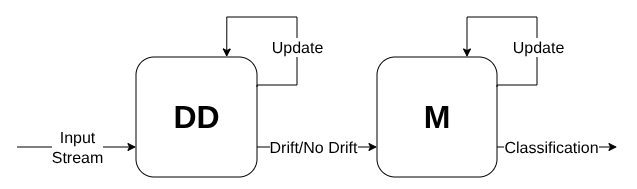
\includegraphics[width=\linewidth]{target_system_threat_model/target architecture.drawio.png}
    \caption{The general architecture of the target system}
    \label{fig:target architecture}
\end{figure}
\todo[color=yellow]{Figure can be improved}

\section{Threat Model}
To systematically evaluate the security of the target system, it is necessary to define the parameters under which an adversary operates. The threat model establishes the attacker's objectives, their level of knowledge about the system, and their practical capabilities within the environment.

\subsection{Attacker Objectives}
The primary objective of an adversary is to compromise the predictive accuracy or operational efficiency of the system as a whole. In this context, this manifests in two distinct ways:
\begin{itemize}
    \item \textit{Forcing False Adaptation}: The attacker aims to deceive the RRBM-DD into signalling a drift when the underlying distribution is stable, causing the Decision Tree to unnecessarily adapt to potentially malicious data, degrading its accuracy or consuming computational resources.

    \item \textit{Impairing Adaptation}: The attacker injects data that masks genuine concept drift in some way, preventing the RRBM-DD from detecting valid shifts and forcing the Decision Tree to rely on an outdated model.
\end{itemize}

\subsection{Attacker Knowledge}
The viability of an attack heavily depends on the adversary's understanding of the target system. The attacker's knowledge can be framed under 3 different assumptions:
\begin{itemize}
    \item \textit{White-Box:} The adversary possesses complete knowledge of the system. This includes but is not limited to the RRBM-DD's exact architecture, its current weights, the size of the mini-batches, and the specific statistical thresholds used in the Granger causality test.
   
    \item \textit{Grey-Box:} The adversary knows the general system architecture (e.g. that an RRBM-DD and a Decision Tree are being used) and the features of the data stream, but lacks access to the internal weights, sliding window states, or exact hyperparameters in real-time.
    
    \item \textit{Black-Box:} The adversary is unaware of the specific detection algorithms or base learner implemented. They can only observe the output predictions and the raw incoming data stream, meaning they must infer further details like the occurrence of a drift signal, based on changes in the system's external behaviour.
\end{itemize}

\subsection{Attacker Capabilities}
In the context of data stream mining, the adversary is assumed to have write access to the data ingestion pipeline, allowing them to manipulate the stream before it enters the predictive system. The adversary's capabilities are defined by the following constraints:
\begin{itemize}
    \item \textit{Feature Manipulation}: The ability to perturb the feature vector $X$ of incoming data points.
    
    \item \textit{Label Flipping}: The ability to alter the ground-truth label $y$ provided to the system.
    
    \item \textit{Injection Budget}: An adversary cannot replace 100\% of the stream, as this would trivially overwrite the system and would likely be flagged by upstream anomaly detection.
\end{itemize}
\chapter{Attack Taxonomy and Objectives}
\label{ch:attack_taxonomy_objectives}

This chapter systematically explores the attack vectors that can be deployed against the target continual learning pipeline. Because the architecture couples a base learner ($M$) with a trainable drift detector ($DD$), its security must be evaluated across multiple dimensions. We introduce a $3 \times 3$ attack matrix, categorising threats along two axes: attacks on the base learner and attacks on the drift detector.\todo[color=green]{Maybe mention something about the maintenance of attacks}

\section{Axis 1: Attacks on the Base Learner ($M$)}
Attacks on the base learner (the Decision Tree) aim to degrade its predictive performance, either during inference or by exploiting retraining.
\begin{itemize}
    \item \textit{Evade $M$}: The adversary crafts perturbations to input features to force a misclassification, bypassing the current decision boundary without altering the model itself. Occurs strictly during the inference phase.

    \item \textit{Poison $M$}: Exploits system adaptation by ensuring corrupted data is included in the retraining buffer when a drift is signalled, forcing $M$ to learn a false concept and degrading its accuracy.

    \item \textit{Backdoor $M$}: A targeted form of poisoning where the adversary injects a feature "trigger" paired with a target label into the retraining buffer. After the update, $M$ behaves normally on clean data but behaves as the attacker specified for inputs containing the hidden trigger.
\end{itemize}


\section{Axis 2: Attacks on the Drift Detector ($DD$)}
Attacks on the RRBM-DD aim to hijack the system's supervisory mechanism, dictating when and if the system adapts.
\begin{itemize}
    \item \textit{Evade $DD$}: Causes misclassification without needing to alter the weights of $DD$. This manifests as either a False Negative (masking real drift) or a False Positive (triggering unnecessary retraining).

    As a stand-alone attack, a stream of False Negatives can be used to stop $M$ from learning, and a stream of False Positives can be used as a form of Denial of Service by causing repeated retraining.

    \item \textit{Poison $DD$}: Exploits the fact that RRBM-DD's trains itself continually. The adversary injects adversarial concepts that bypass the network's robust gradient and noise filters, corrupting its understanding of the distribution. 

    This can be used alone to increase or decrease the detector's tolerance to changes, causing blindness or hypersensitivity to real drift, respectively.

    \item \textit{Backdoor $DD$}: Plants a hidden trigger within the RRBM-DD's latent representation by exploiting its online updating mechanism. This establishes a targeted vulnerability without corrupting the detector's baseline performance.
    
    This alone can grant an attacker precise, on-demand control over the system, allowing them to dictate exactly when a drift is detected and when a retraining cycle is initiated or suppressed.
\end{itemize}

\section{The Maintenance Principle}
\label{sec:maintenance principle}
Because the target architecture relies on a trigger-based adaptation mechanism, any malicious payload injected into the system is inherently temporary. Continual learning systems naturally evolve; therefore, even if an attacker successfully poisons the base learner ($M$), subsequent natural concept drift will trigger a new retraining cycle and overwrite the compromised model.

Therefore, any poisoning or backdoor placed in either $DD$ or $M$ must be actively maintained. When attacking $DD$, the adversary must continuously inject the adversarial distribution into the stream to prevent the neural network from healing and relearning the true data distribution. When attacking $M$, the adversary must protect the compromised model by suppressing future drift signals to prevent $M$ from retraining. This suppression can be achieved by actively evading $DD$ (forcing false negatives), poisoning $DD$ to raise its tolerance, or utilising a backdoor in $DD$ to dictate its signalling behaviour.

\subsection{Meaningful Single-Component Attacks}
...\todo[color=green]{Write a subsection here (include attacks that require no DD manipulation - ride real drift signal)}

\section{Compound Attacks: The Matrix of Combinations}
By combining the three strategies for $M$ (Evade, Poison, Backdoor) with the three strategies for $DD$, we yield nine potential compound attacks. The following subsections categorise these combinations based on their practical viability and threat level.

\subsection{The Primary Threats}
These combinations are both viable and present a threat.\todo[color=green]{Break into more subcategories}
\begin{itemize}
    \item \textit{Evade $DD$ + Poison $M$}: The attacker injects data that causes $DD$ to falsely signal a drift. $M$ is subsequently retrained on a batch of poisoned instances injected concurrently by the attacker. The attacker must then maintain this poisoned state using the methods discussed in~\cref{sec:maintenance principle}.

    \item \textit{Evade $DD$ + Backdoor $M$}: Mechanically similar to the attack above, but rather than degrading general accuracy, the attacker implants a specific feature trigger into $M$ during the forced retraining cycle.

    \item \textit{Poison $M$ + Poison $DD$}: During a retraining cycle (triggered either by an evasion of $DD$ or a genuine drift signal), the attacker uses poisoned instances to corrupt $M$. Concurrently, these instances must circumvent $DD$'s robustness measures, manipulating its internal representation so it accepts the adversarial distribution as normal. The state of $DD$ must then be maintained using the methods laid out in~\cref{sec:maintenance principle}.

    \item \textit{Backdoor $M$ + Poison $DD$}: Following the same methodology as the attack above, the attacker poisons $DD$ (and maintains it) to secure the system's state. But they implant a specific latent trigger in $M$ during retraining rather than just degrading its general accuracy.

    \item \textit{Poison $DD$ + Evade $M$}: To execute a high volume of evasion attacks against $M$, the attacker must prevent these adversarial inputs from triggering a drift signal. The attacker first poisons $DD$, raising its tolerance to change. With the detector effectively blinded, the attacker can feed crafted, highly perturbed evasion inputs to $M$ without fear of triggering a defensive retraining cycle.
    
    \item \textit{Backdoor $DD$ + Poison $M$}: The attacker first establishes a latent trigger in $DD$. When the attacker is ready to poison $M$, they activate the $DD$ backdoor to fire a drift signal exactly when their poisoned payload enters the window, effectively guaranteeing $M$ retrains on the malicious data.
\end{itemize}

\subsection{Pointless or Impractical Combinations}
These combinations represent conflicting operational objectives or technical infeasibility.
\begin{itemize}
    \item \textit{Evade $M$ + Evade $DD$}: If the attacker's goal is to cause a misclassification on $M$ during inference, evading $DD$ adds no value. (The exception is where a mass evasion campaign on $M$ is the goal).

    \item \textit{Backdoor $DD$ + Evade $M$}: Establishing a backdoor in a complex generative model like the RRBM-DD requires a considerable amount of effort. Using that backdoor merely to facilitate instance-level evasion on $M$ (a binary Decision Tree) is a waste of resources. 

    \item \textit{Backdoor $DD$ + Backdoor $M$}: This requires the adversary to simultaneously train two entirely distinct, hidden triggers into two radically different architectures using the same data stream. Optimising for both simultaneously, without them interfering with one another, is likely practically impossible.
\end{itemize}
\chapter{Implementation}
\label{ch:implementation}

This chapter describes how the target system of \cref{ch:target_system_threat_model}, our evaluation pipeline and our attacks are realised in code. Because Kuppa and Le-Khac~\cite{Kuppa_2022} release neither code nor a precise specification of several components, we first reimplement their Contrastive NCM detector and confirm that the reimplementation reproduces their reported behaviour. We then build the coupled adaptive system in which the detector supervises a downstream base learner, and describe the design decisions that this required. Four of these decisions complete components that the paper leaves under-specified and each was surfaced by a concrete failure of a naive implementation rather than chosen a priori. We frame them as filling gaps in the paper's intended architecture, not as corrections to it. The chapter closes with the implementation of the attacks selected for evaluation in \cref{ch:attack_taxonomy_objectives}.

\section{Datasets and Preprocessing}
\label{sec:impl-data}
We evaluate on CICIDS2017, a widely used intrusion-detection benchmark of labelled bidirectional network flows captured over five working days~\cite{Sharafaldin_2018}. We use the Engelen-corrected release of CICIDS2017~\cite{Engelen_2021}, which repairs documented errors in the original dataset's labelling and feature-extraction pipeline. Kuppa and Le-Khac~\cite{Kuppa_2022} report using this same correction, although their testbed description matches the larger CSE-CIC-IDS2018 dataset\footnote{A corrected CSE-CIC-IDS2018 also exists~\cite{Liu_2022}, but post-dates~\cite{Kuppa_2022} and is not the correction they cite.}. Therefore we read their evaluation as using the same corrected CICIDS2017. However, the comparison in \cref{sec:impl-repro-results} is still indicative rather than exact because the reference implementation, the test-set composition, and the feature subset all remain unspecified.

The five daily captures are concatenated in their natural order. We discard flow-identifier columns (the flow identifier, source and destination addresses and ports, and the timestamp) so that the detector cannot key on artefacts of the capture rather than on actual traffic behaviour. We also consolidate the fine-grained attack labels into their parent families (for example, the several denial-of-service variants into a single \texttt{DoS} class). Non-finite feature values are replaced, all-empty columns are dropped, the remaining gaps are mean-imputed, and the features are standardised. We are left with a $77$-dimensional input space over seven traffic classes. Kuppa and Le-Khac~\cite{Kuppa_2022} report a $72$-dimensional feature set but do not specify which columns they retain, so we could not match their exact feature space; this is a concrete instance of the unpublished preprocessing noted above.

To simulate concept drift we withhold a subset of classes as \textit{novel}: these never appear in the initial training data and first arrive partway through the stream, while the remaining \textit{known} classes train the initial detector and base learner. Our main experiments withhold \texttt{DoS} and \texttt{PortScan}; a robustness variant withholds \texttt{DoS} and \texttt{DDoS} (\cref{ch:evaluation}). The stream preserves the natural Monday-to-Friday ordering rather than being shuffled, so novel traffic arrives at its true point in time mirroring a real-world scenario.

\section{Reimplementing and Reproducing the Contrastive NCM Detector}
\label{sec:impl-reproduction}

\subsection{Reimplementation}
\label{sec:impl-reimpl}
Because no reference implementation is published, we reimplement the detector of \cref{sec:contrastive_ncm} in PyTorch directly from the paper's specification~\cite{Kuppa_2022}. The embedding network is an autoencoder trained jointly on a mean-squared reconstruction loss and the supervised contrastive loss, with temperature $\tau = 0.1$; it maps the $77$-dimensional input to a $32$-dimensional latent space through a single $64$-unit hidden layer. On these embeddings we fit the Nearest Class Mean classifier with the hybrid distance of \cref{eq:hybrid-distance} ($\lambda_1 = 0.1$), taking each class prototype to be the mean latent vector of its training samples. Concept discovery accumulates the telescoping displacement of successive drifted-batch means as in \cref{eq:concept-threshold}. Following the paper we train the encoder network with the Adam optimiser at a learning rate of $10^{-4}$ for $300$ epochs, on its $25/75$ train--test split.

Three components are deliberately left open at this stage because the paper does not specify them: the calibration of the two thresholds (\cref{sec:impl-calibration}), the policy for retaining past concepts (\cref{sec:impl-retrain}), and the exact coupling to a downstream classifier (\cref{sec:impl-coupled}). We fix the reimplementation against the paper before introducing any of them.

\subsection{Reproduction}
\label{sec:impl-repro-results}
We validate the reimplementation on the paper's drift-detection protocol: a subset of classes is withheld from training, their test-set samples form the drifted (positive) class and the other classes the negatives. Matching the paper's ``two classes dropped'', chosen at random over five runs, we compare precision, recall and $F_1$ directly against its reported values (\cref{tab:impl-reproduction}). The plain-autoencoder baseline reproduces almost exactly ($F_1 = 0.788$ against $0.777$) and the contrastive detector lands lower ($0.887$ against $0.942$); a threshold-free check agrees, our AUROC of $85.1$ tracks the same shortfall against the paper's $89.8$. The gap is most plausibly caused by the details the paper leaves unspecified (discussed in \cref{sec:impl-data}), not by the detector itself. The reproduction preserves the paper's ordering, the proposed method ahead of the autoencoder baseline.

\begin{table}[h]
\centering
\caption{Reproduction of the held-out-class drift-detection benchmark at the paper's ``two classes dropped'' setting: our precision, recall and $F_1$ against the values reported by Kuppa and Le-Khac~\cite{Kuppa_2022} (ours averaged over five random two-class withholdings). The plain-autoencoder baseline reproduces almost exactly on $F_1$; the contrastive detector lands modestly lower, and both of our detectors trade precision for recall relative to the paper.}
\label{tab:impl-reproduction}
\begin{tabular}{llccc}
\toprule
Method & Source & Precision & Recall & $F_1$ \\
\midrule
\multirow{2}{*}{Contrastive NCM (proposed)} & Ours              & 0.815 & 0.979 & 0.887 \\
                                            & Kuppa and Le-Khac~\cite{Kuppa_2022} & 0.965 & 0.921 & 0.942 \\
\midrule
\multirow{2}{*}{Plain AE + NCM}             & Ours              & 0.666 & 0.979 & 0.788 \\
                                            & Kuppa and Le-Khac~\cite{Kuppa_2022} & 0.788 & 0.766 & 0.777 \\
\bottomrule
\end{tabular}
\end{table}


The figure above establishes that the reimplementation detects drift as the paper's detector does; they say nothing about its \textit{adversarial robustness}, which is the property for which the contrastive detector was originally proposed. We therefore also run the paper's instance-based poisoning experiment, where a growing fraction of adversarially perturbed novel samples is injected into training, and the contrastive detector's accuracy degrades gracefully with the injection ratio, reproducing the trend the paper reports. We stress that this is only a qualitative check. The paper's headline claim is comparative -- that the Contrastive NCM detector is more robust than its baselines -- and we do not cleanly reproduce that, because the plain-autoencoder baseline sits at the balanced-accuracy floor throughout. We also do not reproduce the paper's concept-based poisoning experiment as it is built on the MAA algorithm~\cite{Kuppa_2019}, a separate black-box manifold-approximation attack whose faithful reimplementation is out of scope.

\section{The Coupled Adaptive System}
\label{sec:impl-coupled}

\subsection{Architecture and Streaming Harness}
\label{sec:impl-harness}
The coupled system realises the architecture of \cref{ch:target_system_threat_model}: the detector $\mathcal{D}$ and base learner $\mathcal{M}$ consume the same stream in parallel. $\mathcal{M}$ classifies each batch while $\mathcal{D}$ monitors it for drift, flagging individual samples (\cref{eq:drift-rule}) and accumulating them in the concept-discovery buffer. When the firing predicate is satisfied (\cref{sec:impl-gate}) the coupling layer assembles a retraining set (\cref{sec:impl-retrain}) and rebuilds the encoder, the class prototypes, and $\mathcal{M}$. A streaming harness drives this loop one batch at a time and records, per batch, the base learner's $F_1$ and per-class false-negative rates, the number of detector and base-learner retraining events, the detector's drift rate on a fixed novel pool, and every firing decision. The harness also exposes the injection hook through which the adversary introduces crafted traffic (\cref{sec:impl-attacks}). The base learner $\mathcal{M}$ that the detector supervises is an MLP with 3 hidden layers ($256$--$128$--$64$ units, \textsc{ReLU}) over the same $77$-dimensional input, with a binary \textsc{benign}/\textsc{attack} output. It is trained under cross-entropy with the Adam optimiser, its initial train running for $100$ epochs at learning rate $10^{-3}$ with inverse-frequency class weights to offset the benign-dominated traffic mixture.

\subsection{Three System Configurations}
\label{sec:impl-configs}
We use three configurations of the coupling, which together form an ablation ladder used throughout \cref{ch:evaluation}:
\begin{itemize}
    \item \textsc{StaticDStaticM}: neither component adapts. $\mathcal{M}$ remains at its initial state and never sees the novel classes. This is the no-adaptation lower bound.
    \item \textsc{StaticDAdaptiveM}: the detector is frozen but $\mathcal{M}$ adapts on each firing event, isolating the composition channel from any drift in the representation itself.
    \item \textsc{AdaptiveDAdaptiveM}: both components adapt on each event. This is the paper-faithful system and the default victim.
\end{itemize}
Fixing which part of the coupling is allowed to adapt lets us attribute observed effects to a specific mechanism rather than to the system as a whole.

\section{Completing the Under-Specified Components}
\label{sec:impl-refinements}
Deploying the detector in a coupled setting forced four design decisions that the paper leaves open. We present each as the naive choice, the concrete failure it produced in our implementation, and the refinement that resolves it. We stress that these complete the paper's intended architecture rather than correct an error in it.

\subsection{The Count-and-Fraction Firing Gate}
\label{sec:impl-gate}
The paper triggers concept discovery based on displacement alone; that is, a new concept is registered once the accumulated displacement crosses $T$. Coupled to a retraining loop, this proved far too eager. In an unattacked run, the system's first concept-discovery event fired on a buffer holding only three attack-labelled drifted samples, rebuilding $\mathcal{M}$ on what could effectively be noise. In other words, a handful of borderline samples can satisfy it long before genuine drift is present.

We therefore gate firing on the \textit{makeup} of the buffer in addition to its displacement. A retraining event fires only when the buffer holds at least a minimum count of attack-labelled drifted samples (we use $500$) and those samples constitute at least a minimum fraction of the buffer (we use $0.3$). These two floors are the count and fraction sub-surfaces of the trigger channel named in \cref{sec:adaptation_cycle}; the trigger-channel attacks of \cref{ch:evaluation} act on them, and \cref{sec:eval-rq3-gate} decomposes their distinct roles.

\subsection{Threshold Calibration}
\label{sec:impl-calibration}
The paper sets the concept threshold $T = 3.5$ a priori, but this value is tied to the scale of its embeddings and does not transfer to ours. We calibrate both thresholds on a held-out sample of known-class data. The drift threshold $T_{drift}$ is set to the $0.90$ quantile of known-class drift scores, fixing the known-class false-positive rate at roughly $10\%$ and giving $T_{drift} = 1.34$. The concept threshold is set by a calibration routine that measures the accumulated drifted-batch displacement (\cref{eq:concept-threshold}) over $200$ seeded runs (each across $20$ random sub-batches of 256 known-class samples) and takes the $0.995$ quantile of the resulting norms, giving $T = 37.84$. The values above are those of the main victim (with novel classes \texttt{DoS} and \texttt{PortScan} withheld); independently-trained detectors calibrate comparable but distinct thresholds under the same rule (the $T_{drift}$ values of the \cref{ch:evaluation} variants span $1.19$--$1.34$). Within a run, $T_{drift}$ is held fixed, while $T$ is recalibrated on the new encoder at each retraining event.

\subsection{Retrain-Set Composition and Encoder Stability}
\label{sec:impl-retrain}
When a retraining event fires the encoder must be rebuilt, and the paper does not specify on what data. The naive choice is retraining on the drifted buffer alone; this destabilises the representation. The encoder specifically reorganises its latent space around the newly discovered concept and known-class performance collapses. This is equivalent to catastrophic forgetting~\cite{French_1999}, where learning a new task erases earlier ones.

Following the rehearsal principle that mitigates forgetting~\cite{Robins_1995}, the coupling layer composes the retraining set from the drifted buffer together with a fixed-size set of per-class exemplars selected via herding (\cref{eq:herding})~\cite{Rebuffi_2017}. We adopt an \textit{accumulate, never evict} policy, meaning once a concept is registered, its exemplars are retained for every subsequent rebuild. This realises the composition channel concretely, and it has a direct consequence for adversarial persistence (\cref{ch:attack_taxonomy_objectives}). The same rehearsal that protects a genuine concept against forgetting protects an adversarial one just as faithfully, preventing the system from ``healing'' on its own once a payload has been registered.

In our implementation both components are rebuilt \emph{from scratch} on a firing event, re-initialised and re-trained under the same protocol used at initialisation, following the paper~\cite{Kuppa_2022}. The base learner $\mathcal{M}$ is re-initialised and trained for $100$ epochs, with inverse-frequency class weights, on the binary set formed from the drifted buffer, the per-class known exemplars, and the accumulated novel exemplars. It is worth noting that the labels used are the ones observed, including any the adversary has forged. The encoder is likewise re-initialised and trained for $300$ epochs under the same contrastive loss on the same data with its multiclass labels, with the drifted buffer capped at $5000$ samples and assigned the newly registered prototype and the known exemplars repeated twice to rebalance the loss against the buffer. Each discovered concept contributes up to $500$ herding-selected exemplars to the accumulated novel set, which under the never-evict policy is retained at every subsequent rebuild.

\subsection{Stream-Side Evaluation}
\label{sec:impl-eval}
Finally, the coupling forces a choice of evaluation surface, and two recur throughout the thesis. Testing $\mathcal{M}$ on a fixed, class-balanced \textit{benchmark} set, aware of the novel classes (\textit{bench} $F_1$), captures its standing accuracy, but this is not what a deployed system experiences. We therefore also evaluate $\mathcal{M}$ on the day's actual stream traffic (\textit{stream} $F_1$), batch by batch, and report end-of-stream (Friday) figures. Throughout, we report per-class false-negative rates alongside aggregate $F_1$, because, as the attacks of \cref{ch:evaluation} show, aggregate $F_1$ can remain almost unchanged while the false-negative rate on a single attack class rises sharply.

With these four refinements in place, the coupled system adapts correctly under genuine drift: on an unattacked run it discovers the novel classes, retrains three times over the week, and reaches a Friday bench $F_1$ of $0.700$, against a no-adaptation floor of $0.207$. This working configuration is the baseline against which \cref{ch:evaluation} measures every attack.

\section{Attack Implementation}
\label{sec:impl-attacks}
We close with the implementation of the attacks selected for evaluation in \cref{ch:attack_taxonomy_objectives}; their results are reported in \cref{ch:evaluation}. We organise them by adversarial \textit{objective} rather than by channel, because a single mechanism can act through more than one channel, and the objective is what the evaluation actually measures. All four attacks are instances of the shared injection model described next.

\subsection{The Injection Model}
\label{sec:impl-injection}
The adversary acts by injecting crafted flows into the stream. We model this as a per-batch \textit{injection} rather than replacement: at injection fraction $p$ the attacker adds $\lfloor\, p\,n_t \,\rfloor$ samples to a batch of $n_t$ genuine samples, so the crafted flows make up a fraction $p/(1+p)$ of the batch (\cref{def:injection_budget}). The injected flows are drawn with replacement from the withheld novel pool, then concatenated into the batch and shuffled; injection is also gated to begin only after the all-benign Monday warm-up. Two further degrees of freedom complete the model. First, the attacker chooses the \textit{label} under which the injected flows are presented, which determines both whether they push the firing gate towards or away from a fire and what $\mathcal{M}$ learns if a rebuild does occur. Second, the injection rate may be varied over the time through a \textit{schedule} function, supporting sustained and time-varying injection. Each attack below is an instance of this model under a particular label and schedule; the feature-space attack of \cref{sec:impl-pgd} additionally perturbs the injected flows themselves.

\subsection{Suppressing Adaptation}
\label{sec:impl-suppress}
The simplest way to deny adaptation is to hold the firing gate shut. The gate's two floors on the drifted samples mean it fires only once at least $500$ of them have accumulated and they make up at least $30\%$ of the buffer (\cref{sec:impl-gate}). The per instance drift threshold, however, is label-independent, meaning a novel sample is flagged as drifted whether the adversary presents it as benign or as attack. Injecting novel flows under a \textit{benign} label therefore admits them to the buffer, inflating its size, while withholding them from the attack-labelled count, which drives the attack fraction below the $0.3$ floor. If this is sustained at a sufficient rate the gate can be held shut for the whole stream, so no concept-discovery event fires, $\mathcal{M}$ is never rebuilt, and the emerging class is never learned. The attack crafts no features, relying only on the ability to inject benign-labelled flows.

\subsection{Forcing Adaptation}
\label{sec:impl-force}
\label{sec:impl-pgd}
Forcing is the dual objective: rather than starving the gate, the adversary drives it past its thresholds to trigger an attacker-timed rebuild -- either earlier than genuine drift would, or on an otherwise stable distribution. Because the gate is a conjunction (\cref{sec:impl-gate}), a forcing attack must satisfy all three conditions at once, and this rules out any displacement-only manoeuvres. Injecting drifted flows under a \textit{benign} label does move the accumulated displacement but, carrying no attack label, such flows fail the count and fraction floors. Forcing therefore requires perturbing flows that are injected under the \textit{attack} label, so that they raise the floors while also displacing the batch mean. We realise this with a feature-space attack.

The feature-space attacks perturb the injected flows directly and come in three variants of increasing sophistication. A \textit{per-sample} variant maximises each flow's individual drift score. It saturates instance level drift \textit{detection}, but because each embedding is pushed independently the batch mean barely moves, so it does \textit{not} force a fire -- this is the basis of the ``fooling detection is not forcing'' result of \cref{sec:eval-rq3-pgd}. A \textit{directional} variant instead pushes every embedding along a single fixed (but random) latent direction, producing a coherent batch-mean shift. This can cross $T$, but only at a large budget, and serves as the naive baseline. The \textit{mean-shift} variant optimises that direction rather than fixing it, and is the efficient forcing attack.

All three variants use projected gradient descent under an $L_\infty$ budget $\epsilon$ (swept in \cref{ch:evaluation}): $50$ steps of step size $\alpha = 2.5\,\epsilon/50$, projecting onto the $\epsilon$-ball at each step and then clipping to the per-feature observed range so the crafted flows stay within plausible feature values. All operate on a fixed attack pool of $2000$ held-out known-class flows. The mean-shift variant perturbs this pool in two opposite latent directions to maximise the separation of the resulting encoded batch means, $\max\|\mu_A-\mu_B\|$; the perturbed flows are injected under the attack label so that they also satisfy the gate's count and fraction floors. Each variant is run white-box, perturbing against the victim detector itself, and grey-box, perturbing against a surrogate detector and transferring the crafted flows to the victim. The surrogate shares the victim's architecture, hyperparameters and withheld classes but is trained on a disjoint partition of the known-class data, sharing no training flows with the victim (\cref{sec:eval-rq3-pgd}). Therefore it models an adversary who knows the system design and the data distribution and trains their own detector, rather than one with access to the victim's data.

\subsection{Poisoning the Base Learner}
\label{sec:impl-poison}
Where suppression and forcing act on \textit{when} $\mathcal{M}$ rebuilds, poisoning targets \textit{what} it rebuilds on. The mechanism is the benign-labelled injection of \cref{sec:impl-suppress}, but at a low rate that doesn't cause the same suppression. It instead rides the genuine mid-week drift event (the Wednesday arrival of the held-out classes). When the real novel class arrives and the system fires, the mislabelled-benign flows the adversary has injected are themselves drifted, so they too are harvested into the concept-discovery buffer and carried into $\mathcal{M}$'s retraining set under the wrong label. $\mathcal{M}$ then learns the novel attack pattern as benign, inflating its per-class false-negative rate while leaving more general accuracy almost unchanged. Suppression and this version of poisoning are therefore two regimes of the same benign-labelled injection -- at a high rate it starves the gate, at a low rate it survives the gate and corrupts the harvested concept. Hence \cref{ch:evaluation} sweeps the injection fraction to expose both.

\chapter{Evaluation}
\label{ch:evaluation}

% Render this chapter's tables and figures inline (where written) rather than letting them float.
\floatplacement{table}{H}
\floatplacement{figure}{H}

This chapter evaluates the coupled adaptive system of~\cref{ch:implementation} against the attacks specified in~\cref{sec:axt-scope}. It is organised around the three research questions of this thesis, relating to: the attack surface the coupling exposes (RQ1), poisoning attacks on the base learner through the composition channel (RQ2), and evasion attacks on the detector through the trigger channel (RQ3). Each is presented as a hypothesis, the results, and a discussion.~\cref{sec:eval-settings} fixes the elements common to every experiment; experimental settings that vary between them are stated in a \textit{Setup} note at the head of each section.

\section{Experimental Settings}
\label{sec:eval-settings}
The victim throughout is the full coupled system, \textsc{AdaptiveDAdaptiveM} of~\cref{sec:impl-configs}, in which both the detector $\mathcal{D}$ and the base learner $\mathcal{M}$ are rebuilt at each concept-discovery event. Two reduced configurations serve as references where an ablation requires them: \textsc{StaticDStaticM}, which never adapts and fixes the no-adaptation floor, and \textsc{StaticDAdaptiveM}, in which the encoder is frozen but $\mathcal{M}$ still rebuilds.

The stream is the Monday--Friday CICIDS2017 trace (Engelen-corrected,~\cref{sec:impl-data}) replayed in temporal order; \texttt{DoS} and \texttt{PortScan} are held out as the two novel classes that arrive mid-week, so that genuine drift is present in every run. The adversary acts through the injection model of~\cref{sec:impl-injection}. Every detector is calibrated by the rule of~\cref{sec:impl-calibration}, but the resulting threshold values depend on the detector's training set and are therefore stated per experiment. We report $F_1$ measures against a fixed novel-class-aware benchmark and per-class false-negative rate (FNR) alongside it.

\section{Baseline Behaviour Under Genuine Drift}
\label{sec:eval-baseline}
\textit{Setup.} The \textsc{AdaptiveDAdaptiveM} victim is trained on the full known-class pool ($T_{drift} = 1.34$, $T = 37.84$), run on the unpoisoned stream and averaged over three seeds.

Before introducing an adversary we confirm that, on an unpoisoned stream, the coupled system adapts to the genuine drift. It discovers \texttt{DoS} as it arrives mid-week (registering it as a new concept and rebuilding once) and recovers to a Friday $F_1$ of $0.71$ against the no-adaptation floor of $0.207$ (\cref{tab:baseline-adaptation}). It does \emph{not}, however, discover \texttt{PortScan}: that class embeds too close to a known prototype to be flagged as drift (\cref{sec:eval-rq2}), so the system adapts to only one of the two novel classes. This run is the reference point for every attack that follows.

\cref{tab:baseline-adaptation} makes this concrete by comparing the full system (\textsc{AdaptiveDAdaptiveM}) to the static floor (\textsc{StaticDStaticM}, where $\mathcal{M}$ never updates), on aggregate $F_1$ and per-class false-negative rate. Both sit at the floor on Monday and Tuesday; once \texttt{DoS} is discovered during Wednesday, the full system's aggregate $F_1$ climbs from $0.207$ to $0.710$ and its \texttt{DoS} false-negative rate falls from $0.881$ to $0.008$, while the static floor stays put all week. However, the \texttt{PortScan} false-negative rate barely moves from the floor's $0.999$ to $0.983$. This is because the system never discovers that class. We report per-class rates throughout for exactly this reason: aggregate $F_1$ alone would hide a whole novel class going undetected.

\begin{table}
\caption{Baseline (no attack) per-day metrics for the static reference and the full system. $F_1$ is measured against a fixed novel-class-aware benchmark and false-negative rate is measured for \texttt{DoS} and \texttt{PortScan}, whose novel instances arrive on Wednesday and Friday respectively.}
\label{tab:baseline-adaptation}
\centering
\begin{tabular}{lcccccc}
\toprule
 & \multicolumn{3}{c}{\textsc{StaticDStaticM}} & \multicolumn{3}{c}{\textsc{AdaptiveDAdaptiveM}} \\
\cmidrule(lr){2-4}\cmidrule(lr){5-7}
Day & $F_1$ & FNR(\texttt{DoS}) & FNR(\texttt{PortScan}) & $F_1$ & FNR(\texttt{DoS}) & FNR(\texttt{PortScan}) \\
\midrule
Mon & 0.207 & 0.881 & 0.999 & 0.207 & 0.881 & 0.999 \\
Tue & 0.207 & 0.881 & 0.999 & 0.207 & 0.881 & 0.999 \\
Wed & 0.207 & 0.881 & 0.999 & 0.346 & 0.640 & 0.995 \\
Thu & 0.207 & 0.881 & 0.999 & 0.710 & 0.008 & 0.983 \\
Fri & 0.207 & 0.881 & 0.999 & 0.710 & 0.008 & 0.983 \\
\bottomrule
\end{tabular}
\end{table}


\clearpage

\section{RQ1 -- The Attack Surfaces of the Coupling}
\label{sec:eval-rq1}
\textit{Hypothesis.} The trigger-dependent coupling exposes attack surfaces that a continuously-updated learner does not. Namely, a trigger channel that decides when rebuilds occur, and a composition channel that decides what data rebuilds use.

The baseline run is itself the evidence. Because $\mathcal{M}$ changes only when the predicate fires (\cref{tab:baseline-adaptation}), the trigger gates all adaptation. This means an adversary who controls whether the predicate fires controls whether $\mathcal{M}$ ever learns the emerging class, and an adversary who controls the buffer at a firing event controls what it learns. A continuously-updated learner offers no such discrete gate; its decision boundary is a moving target that dilutes any single injection. The remainder of the chapter exploits exactly these two surfaces: RQ2 attacks the composition channel and RQ3 the trigger channel. Both are properties of the coupling and both are invisible to a detector-only evaluation.
\clearpage

\section{RQ2 -- The Composition Channel: Poisoning and Backdooring the Base Learner}
\label{sec:eval-rq2}
\textit{Hypothesis.} The composition channel (the data a firing event retrains on) lets the adversary corrupt $\mathcal{M}$ through its retraining set.

\textit{Setup.} The victim is the full-data \textsc{AdaptiveDAdaptiveM} ($T_{drift} = 1.34$, $T = 37.84$). The adversary acts only through the benign-labelled injection of~\cref{sec:impl-injection}; its rate, schedule, and feature perturbations vary by experiment and are stated where each is introduced. All results average three seeds.

Contrary to the hypothesis, a base learner retrained from scratch to convergence \emph{resists} this poisoning. Sweeping a benign-labelled injection of novel \texttt{DoS} flows over $p \in \{0, 5, \dots, 35\}\%$ and riding the genuine mid-week drift event, so that the mislabelled flows are placed into $\mathcal{M}$'s retraining set, leaves the \texttt{DoS} false-negative rate essentially at its clean value across the low and mid budgets ($0.019$ at $p = 0$, $0.014$ at $5\%$, $0.033$ at $20\%$ --~\cref{tab:attack-fri-summary}). The mislabelled flows are a down-weighted minority in a set dominated by correctly-labelled exemplars, so the rebuilt $\mathcal{M}$ still classifies \texttt{DoS} correctly. Persistence does not help: a \emph{durable} variant that injects only around the fire and then stops, lodging its payload in the never-evict exemplar memory, is absorbed just the same. The large per-class damage that a single under-trained rebuild would expose is therefore an artefact of the retraining recipe, not of the coupling; an encoder-freeze ablation (\textsc{StaticDAdaptiveM}) confirms there is no representation-level poisoning to relocate, the frozen-encoder false-negative rate being no lower than the adapting one.

\begin{table}
\caption{Friday end-of-stream attack effect on the full coupled adaptive IDS (\textsc{AdaptiveDAdaptiveM}). Values are mean $\pm$ std across three seeds.}
\label{tab:attack-fri-summary}
\resizebox{\textwidth}{!}{
\begin{tabular}{llcccl}
\toprule
 & Poison \% & Fri $F_1$ & Fri FNR(\texttt{DoS}) & Fri FNR(\texttt{PS}) & Retrains \\
System &  &  &  &  & \\
\midrule
\textsc{StaticDStaticM} & ref & 0.207 $\pm$ 0.000 & 0.881 $\pm$ 0.000 & 0.999 $\pm$ 0.000 & 0 \\
\textsc{AdaptiveDAdaptiveM} & 0 & 0.710 $\pm$ 0.000 & 0.008 $\pm$ 0.000 & 0.983 $\pm$ 0.000 & 1 \\
\textsc{AdaptiveDAdaptiveM} & 5 & 0.726 $\pm$ 0.034 & 0.014 $\pm$ 0.006 & 0.903 $\pm$ 0.137 & 1.3$\pm$0.5 \\
\textsc{AdaptiveDAdaptiveM} & 15 & 0.820 $\pm$ 0.053 & 0.030 $\pm$ 0.003 & 0.529 $\pm$ 0.205 & 2.0$\pm$0.0 \\
\textsc{AdaptiveDAdaptiveM} & 20 & 0.821 $\pm$ 0.053 & 0.033 $\pm$ 0.002 & 0.508 $\pm$ 0.175 & 2.0$\pm$0.0 \\
\textsc{AdaptiveDAdaptiveM} & 25 & 0.207 $\pm$ 0.000 & 0.881 $\pm$ 0.000 & 0.999 $\pm$ 0.000 & 0.0$\pm$0.0 \\
\textsc{AdaptiveDAdaptiveM} & 30 & 0.680 $\pm$ 0.006 & 0.055 $\pm$ 0.011 & 1.000 $\pm$ 0.000 & 1.0$\pm$0.0 \\
\textsc{AdaptiveDAdaptiveM} & 35 & 0.702 $\pm$ 0.001 & 0.006 $\pm$ 0.001 & 1.000 $\pm$ 0.000 & 1.0$\pm$0.0 \\
\bottomrule
\end{tabular}
}
\end{table}

So, the boundary cannot be moved against the genuine class, but it can be circumvented. The channel admits a backdoor, which succeeds precisely because it does not contend with the clean decision boundary. Rather than just mislabelling \texttt{DoS} as benign, the adversary also stamps them with a small feature-space trigger, teaching $\mathcal{M}$ that ``\texttt{DoS}-features $+$ trigger $\Rightarrow$ benign''. The trigger is inert on an un-poisoned learner -- it moves the \texttt{DoS} false-negative rate from $0.012$ to $0.014$ -- but after the backdoor is planted a \emph{triggered} \texttt{DoS} flow evades $\mathcal{M}$ with false-negative rate $0.69$, while \emph{clean} \texttt{DoS} is still caught (with false-negative rate $0.03$). The backdoor is also durable: the adversary injects only around the genuine mid-week fire and then stops, yet the backdoor persists regardless of any further retrains. This is because of all the harvested concept exemplars that carry the trigger being replayed into every subsequent rebuild -- the never-evict exemplar memory (\cref{sec:impl-retrain}) turned against the system. An ablation that disables this memory isolates its role (\cref{tab:rq2-backdoor}). With the harvested exemplars retained (accum=500) the triggered false-negative rate stays consistently high ($0.687 \pm 0.096$), whereas disabling them (accum=0) leaves the same mean ($0.679$) but makes persistence highly seed-dependent ($\pm 0.454$). Therefore, we can confirm that the never-evict memory is what makes the backdoor reliable over time. That is, without the replayed exemplars, whether a later clean rebuild washes the shortcut out is left to chance. Here, the robust learner resists having its boundary moved, but not having a hidden shortcut installed beside it.

\begin{table}
\caption{Backdooring the base learner through the composition channel. Benign-labelled \texttt{DoS} flows carrying a fixed feature-space trigger are injected (sustained, or poison-then-clean) and harvested into the retraining set. A backdoor is implanted when the false-negative rate on triggered \texttt{DoS} is high while clean \texttt{DoS} FNR and overall $F_1$ are unchanged. Values are mean $\pm$ std across three seeds and the accum=0 row disables the never-evict memory.}
\label{tab:rq2-backdoor}
\resizebox{\textwidth}{!}{
\begin{tabular}{lrrrr}
\toprule
 & Friday $F_1$ & FNR(Clean \texttt{DoS}) & FNR(Triggered \texttt{DoS}) & Retrains \\
Condition &  &  &  &  \\
\midrule
Clean & 0.787 $\pm$ 0.055 & 0.012 $\pm$ 0.005 & 0.014 $\pm$ 0.005 & 2.333 $\pm$ 1.247 \\
Backdoor sustained & 0.387 $\pm$ 0.254 & 0.588 $\pm$ 0.414 & 0.846 $\pm$ 0.109 & 0.333 $\pm$ 0.471 \\
Backdoor & 0.850 $\pm$ 0.051 & 0.034 $\pm$ 0.005 & 0.687 $\pm$ 0.096 & 2.333 $\pm$ 0.471 \\
Backdoor (accum=500) & 0.850 $\pm$ 0.051 & 0.034 $\pm$ 0.005 & 0.687 $\pm$ 0.096 & 2.333 $\pm$ 0.471 \\
Backdoor (accum=0) & 0.747 $\pm$ 0.041 & 0.014 $\pm$ 0.015 & 0.679 $\pm$ 0.454 & 1.333 $\pm$ 0.471 \\
\bottomrule
\end{tabular}
}
\end{table}


Beyond what the rebuilt $\mathcal{M}$ learns, the channel exposes control over whether it is rebuilt at all. Because the firing gate counts attack-labelled drifted samples (\cref{sec:impl-gate}) and benign-labelled flows are drifted but not attack-labelled, a sufficient injection dilutes the buffer below the gate and starves retraining. At the knife-edge fraction $p = 25\%$ the system never fires for the whole stream, and $F_1$ collapses to the no-adaptation floor of $0.207$ with both novel classes left unlearned. The collapse is sharp and non-monotonic ($p = 20\%$ and $p = 30\%$ still fire).

A final finding is structural rather than adversarial: the detector is blind to one of the two novel classes. \texttt{PortScan} embeds close to a known prototype: only $\sim$$2.5\%$ of its flows exceed $T_{drift}$. Therefore, it is rarely flagged as drifted, never registered as a concept, and never learned; its false-negative rate stays relatively high ($0.56$--$1.0$) in every condition, attacked or not. Even on the clean stream the system discovers only \texttt{DoS}, silently failing to adapt to a whole novel attack class. This is a limitation of the proposed detector's drift mechanism that only a coupled, stream-side evaluation surfaces.

RQ2 resolves into a sharper claim than the hypothesis stated. The composition channel resists boundary poisoning, even when mislabelled flows end up in the never-evict memory they are simply absorbed. What the channel exposes instead is two things the robust learner here cannot defend against on its own: a backdoor that installs a trigger-activated shortcut beside the clean boundary and persists through the exemplar memory, and control over whether the system adapts at all (the $p = 25\%$ suppression collapse, compounded by the \texttt{PortScan} blind spot the detector creates unaided). Thus, the composition channel is exploitable, not by corrupting what $\mathcal{M}$ has learned, but by adding to it, or by deciding whether it learns (which we discuss further in~\cref{sec:eval-rq3}).
\clearpage

\section{RQ3 -- The Trigger Channel: Forcing and Suppression Trade-Offs}
\label{sec:eval-rq3}
\textit{Hypothesis.} The detector can be forced to fire when it should not, or suppressed when it should, and the firing floors that resist one failure mode enable the other.

\textit{Setup.} RQ3 spans two harnesses. The firing-gate ablation (\cref{sec:eval-rq3-gate}) uses the full-data victim ($T = 37.84$). The transfer study (\cref{sec:eval-rq3-pgd,sec:eval-rq3-force}) trains the victim on a stratified $75\%$ of the known-class pool ($T = 39.29$) so that its grey-box surrogate can be trained on the disjoint $25\%$, sharing no training flows with the victim. The feature-space PGD uses an $L_\infty$ budget swept over $\epsilon \in \{0.1, 0.25, 0.5, 1.0, 2.0\}$, white-box against the victim and grey-box across three independently-seeded surrogates. All results are averaged over three seeds.

\subsection{Forcing Per-Sample Detection}
\label{sec:eval-rq3-pgd}
We separate two things that are easily conflated: making the detector \emph{flag} a sample as drifted, and making the coupled system \emph{fire} a concept-discovery event. A white-box PGD attack on the per-sample drift score saturates detection trivially -- the flag rate on perturbed known-class flows rises from a clean $0.10$ to $1.0$ by $\epsilon = 0.5$ (\cref{fig:eval-rq3-pgd}). But transfer to grey-box is weak; crafted on a data-disjoint surrogate, the same perturbations move the victim's flag rate to only $\sim0.32$ at $\epsilon = 0.5$, rising to at most $0.60$ at $\epsilon = 2.0$. Furthermore, saturating per-sample detection does not necessarily force a fire. Injected in a stable pre-drift window these flows leave the concept-discovery accumulator below $T$ and trigger no events (for both white-box and grey-box), because firing depends on the displacement of the drifted-batch mean, not on individual flags.

\begin{figure}[H]
    \centering
    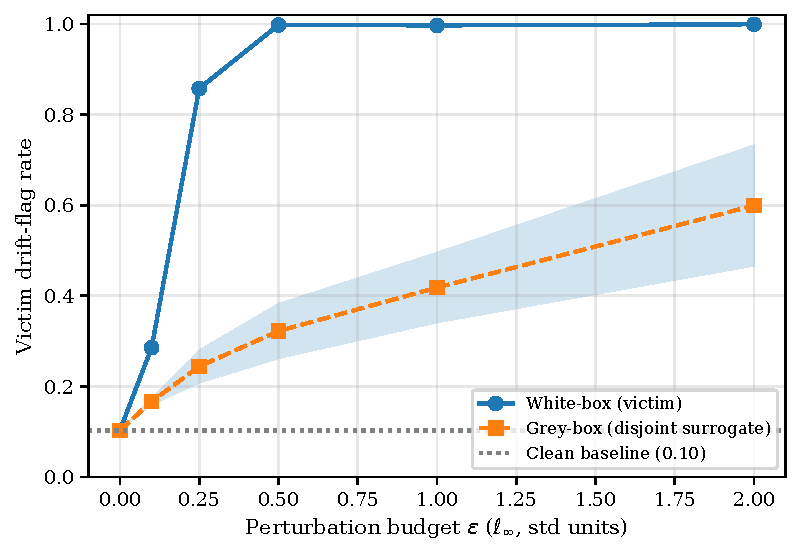
\includegraphics[width=0.7\linewidth]{../experiments/contrastive_ncm/figures/rq3_pgd_false_positive.pdf}
    \caption{PGD false-positive attack on per-sample detection: fraction of perturbed known-class flows the victim flags as drifted versus the $L_\infty$ budget, white-box against the victim and grey-box via surrogate transfer.}
    \label{fig:eval-rq3-pgd}
\end{figure}

\subsection{Forcing the Concept Trigger}
\label{sec:eval-rq3-force}
Forcing therefore requires displacing the batch mean coherently. Naively applying coherent perturbations along a random direction fails. Even white-box at $\epsilon = 2.0$ the accumulated displacement reaches only $29.5$, short of the required threshold $T = 39.3$, and forces no fire. This is what initially looked like robustness. However, we conclude that it is not; it is a weak attack. An aimed mean-shift attack, which optimises two opposing perturbations to maximise the separation of the encoder's batch means, crosses $T$ at $\epsilon \ge 1.0$, reaching displacements of $47$ at $\epsilon = 1.0$ and $92$ at $\epsilon = 2.0$ (\cref{tab:rq3-pgd-meanshift}). Thereby forcing a concept-discovery event white-box.

\begin{table}
\caption{Accumulator attack via direct latent mean-shift: PGD jointly optimises two pools to maximise the separation of their drifted-batch means (the quantity the concept-discovery accumulator integrates), rather than pushing along a fixed random direction. A fire is forced only if the displacement exceeds $T$.}
\label{tab:rq3-pgd-meanshift}
\centering
\begin{tabular}{lccccr}
\toprule
 & Flag A & Flag B & Displacement & Threshold ($T$) & Forces fire? \\
$L_\infty$ budget ($\epsilon$) &  &  &  &  &  \\
\midrule
0.10 & 0.23 & 0.11 & 18.0 & 39.3 & False \\
0.25 & 0.75 & 0.17 & 26.1 & 39.3 & False \\
0.50 & 0.77 & 0.86 & 25.6 & 39.3 & False \\
1.00 & 1.00 & 1.00 & 47.1 & 39.3 & True \\
2.00 & 1.00 & 1.00 & 91.5 & 39.3 & True \\
\bottomrule
\end{tabular}
\end{table}


The most consequential result is that this attack transfers. Crafted against a data-disjoint surrogate and evaluated on the victim, the mean-shift retains roughly $70\%$ of its white-box displacement -- $33$ at $\epsilon = 1.0$ and $65$ at $\epsilon = 2.0$ (\cref{tab:rq3-pgd-meanshift-greybox}). That clears $T = 39.3$ and forces a fire at $\epsilon = 2.0$ while at $\epsilon = 1.0$ the transferred displacement falls just short. This stands in sharp contrast to per-sample detection, which transferred poorly ($\le 60\%$): a per-sample flag requires every sample to individually clear the threshold, which is brittle across two independently-trained encoders. Whereas, the trigger fires on a batch mean and averaging launders the per-sample transfer noise, leaving the coherent direction both encoders agree on. The batch-mean statistic the detector adopts for stability is precisely what makes the trigger grey-box forceable.

\begin{table}
\caption{Grey-box mean-shift transfer. Two pools are optimised against a disjoint surrogate (trained on a held-out 40 percent of the known-class pool, with no flows shared with the victim) and the displacement of their drifted-batch means is measured on the victim. Reported are the mean and std of the transferred displacement over three surrogate seeds and the number of seeds whose transfer forces a victim concept-discovery fire. A fire requires the displacement to exceed $T$ (compare the white-box mean-shift,~\cref{tab:rq3-pgd-meanshift}).}
\label{tab:rq3-pgd-meanshift-greybox}
\centering
\begin{tabular}{lrrr}
\toprule
 & Displacement & Threshold ($T$) & Seeds forcing fire \\
$L_\infty$ budget ($\epsilon$) &  &  &  \\
\midrule
0.10 & 11.1 $\pm$ 0.7 & 39.3 & 0/3 \\
0.25 & 18.3 $\pm$ 1.1 & 39.3 & 0/3 \\
0.50 & 20.7 $\pm$ 1.6 & 39.3 & 0/3 \\
1.00 & 33.1 $\pm$ 2.0 & 39.3 & 0/3 \\
2.00 & 65.0 $\pm$ 3.8 & 39.3 & 3/3 \\
\bottomrule
\end{tabular}
\end{table}


The caveat is the budget. Grey-box forcing requires $\epsilon = 2.0$ here, a large, unconstrained $L_\infty$ perturbation in standardised-feature units that would almost certainly distort flows beyond what protocol constraints permit; a feature-constrained mean-shift would raise the bar further and is left to future work. Within the adopted grey-box threat model, however, the conclusion stands: the concept trigger is forceable, not robust, and the attack is bounded only by the perturbation budget.

\subsection{Decomposing the Firing Gate}
\label{sec:eval-rq3-gate}
The firing predicate is made up of three conjuncts -- displacement, count, and fraction (\cref{sec:axt-surface}). To attribute the system's behaviour to the individual floors we ablate the count and fraction conditions independently, across \texttt{displacement-only} (the paper's rule, neither floor), \texttt{count-only}, \texttt{fraction-only}, and the \texttt{full} gate we propose.

\begin{table}
\caption{Gate ablation (forcing): pre-drift injection of true-labelled novel flows under the four decomposed firing gates of the count/fraction 2x2. Values reported are mean $\pm$ std over seeds.}
\label{tab:rq3-gate-forcing}
\centering
\begin{tabular}{llr}
\toprule
 &  & Forced fires \\
Gate & Poison \% &  \\
\midrule
\multirow[t]{4}{*}{Displacement-only} & 2\% & 0.667 $\pm$ 0.943 \\
 & 5\% & 14.667 $\pm$ 2.867 \\
 & 10\% & 5.000 $\pm$ 2.160 \\
 & 20\% & 0.000 $\pm$ 0.000 \\
\cline{1-3}
\multirow[t]{4}{*}{Count-only} & 2\% & 0.333 $\pm$ 0.471 \\
 & 5\% & 1.667 $\pm$ 0.943 \\
 & 10\% & 2.333 $\pm$ 0.943 \\
 & 20\% & 0.000 $\pm$ 0.000 \\
\cline{1-3}
\multirow[t]{4}{*}{Fraction-only} & 2\% & 0.000 $\pm$ 0.000 \\
 & 5\% & 0.000 $\pm$ 0.000 \\
 & 10\% & 0.000 $\pm$ 0.000 \\
 & 20\% & 0.000 $\pm$ 0.000 \\
\cline{1-3}
\multirow[t]{4}{*}{Full} & 2\% & 0.000 $\pm$ 0.000 \\
 & 5\% & 0.000 $\pm$ 0.000 \\
 & 10\% & 0.000 $\pm$ 0.000 \\
 & 20\% & 0.000 $\pm$ 0.000 \\
\bottomrule
\end{tabular}
\end{table}


\begin{table}
\caption{Gate ablation (suppression): benign-labelled injection at p=25\% during genuine drift under the four decomposed firing gates of the count/fraction 2x2. Reported values are the mean $\pm$ std over seeds.}
\label{tab:rq3-gate-suppression}
\centering
\begin{tabular}{lrr}
\toprule
 & Fri $F_1$ & Retrains \\
Gate &  &  \\
\midrule
Displacement-only & 0.620 $\pm$ 0.036 & 134.667 $\pm$ 22.366 \\
Count-only & 0.207 $\pm$ 0.000 & 0.000 $\pm$ 0.000 \\
Fraction-only & 0.207 $\pm$ 0.000 & 0.000 $\pm$ 0.000 \\
Full & 0.207 $\pm$ 0.000 & 0.000 $\pm$ 0.000 \\
\bottomrule
\end{tabular}
\end{table}


Against forcing (\cref{tab:rq3-gate-forcing}, pre-drift injection of true-labelled flows), the two floors are not equal. The fraction floor alone blocks every forced fire at every budget, because at low injection the attacker's flows are only a small fraction of the drifted buffer which is already padded by the detector's own false positives, so the $0.3$ threshold is never reached. The count floor reduces the efficacy of forcing. It cuts forced fires from $14.7$ to $1.7$ at $p = 5\%$, but it alone is not sufficient since the $500$ samples it demands are within a determined attacker's budget. The full gate, exactly like fraction-only, is completely immune.

Against suppression (\cref{tab:rq3-gate-suppression}, benign injection at $p = 25\%$), the picture inverts. Either floor alone suffices to make the system suppressible. The \texttt{count-only}, \texttt{fraction-only}, and \texttt{full} gates all collapse to the no-adaptation floor ($F_1 = 0.207$, zero retrains), while only \texttt{displacement-only} keeps adapting. However, it does so pathologically, firing approximately $135$ times on the injected noise, and is in turn the most forceable gate of all. The only configuration we examine that resists suppression is the one that cannot resist forcing.

The ablation demonstrates the trade-off of this trigger-gated adaptation mechanism. The suppression vector is over-determined. Any floor placed on the buffer's makeup to resist forcing or premature firing simultaneously hands the adversary a way to hold the buffer below it and starve adaptation. The two floors are defeated by different mechanisms -- the fraction floor by direct dilution (benign flows drive the attack fraction below $0.3$), the count floor is more subtle. Because the displacement accumulator is only reset when the trigger is fired (\cref{eq:concept-accumulator}), a gate that withholds firing lets it telescope into a stationary regime in which $\|\Delta\|$ stays below $T$ even after the count is satisfied. Resetting or windowing the accumulator on gated crossings could be implemented as mitigations, but we leave this to future work. The design implication is stark: under makeup-based gating, making the trigger harder to force and harder to suppress are in direct tension.

\section{Summary}
\label{sec:eval-summary}
The three research questions resolve as follows. RQ1: the trigger-dependent coupling exposes a trigger channel and a composition channel that gate all adaptation, and both are invisible to the detector-only evaluation the literature uses. RQ2: the composition channel \emph{resists} boundary poisoning but it does \emph{not} resist a backdoor, which installs a trigger-activated shortcut beside the clean boundary and persists through the exemplar memory; the same channel also decides whether $\mathcal{M}$ adapts at all (the $p = 25\%$ suppression collapse), compounded by a structural blind spot in which the detector never discovers \texttt{PortScan}. RQ3: the firing trigger is forceable, not robust. An aimed mean-shift attack forces a concept-discovery event both white-box and grey-box (retaining roughly $70\%$ of its displacement against a data-disjoint surrogate); and the gate ablation shows the two firing floors are over-determined, so any floor that resists forcing simultaneously enables suppression. Across all three, the throughline is that coupling a robust detector to a base learner does not make the system robust: the security is further decided at the coupling, a conclusion~\cref{ch:conclusion} draws together.

% We note for completeness that a \emph{flipped-label} manufactured-novelty payload --- attack flows presented under a wrong novel label --- is blocked by the fraction floor at every budget, so an attacker cannot register an arbitrary spurious concept on demand. The complementary \emph{durable}-poison case of~\cref{sec:axt-maintenance} --- poisoning at a damaging rate then running clean, so the payload persists via the never-evict exemplar memory --- is examined directly for the composition channel in~\cref{sec:eval-rq2}.

\chapter{Conclusion}
\label{ch:conclusion}

We set out to evaluate Kuppa and Le-Khac's Contrastive NCM drift detector~\cite{Kuppa_2022} not in isolation, as the literature does, but coupled to the downstream base learner it is meant to supervise -- the configuration in which it would actually be deployed. That coupling, not the detector's representation, is where the security of the system is decided.

Our central finding is that the coupling exposes the adversary to the system's adaptation rather than to its learned decision boundary directly. That is, whether and when the base learner is rebuilt, and what is added to it at a rebuild. Three results make the case. First (RQ1), because the base learner changes only at discrete concept-discovery events, an adversary who controls the firing predicate, or the buffer at a fire, controls what the learner learns and if it learns at all; a continuously-updated learner offers no such gate. Second (RQ3), the firing trigger is \emph{forceable and not robust}: an aimed feature-space mean-shift forces a concept-discovery event both white-box and grey-box, retaining roughly $70\%$ of its displacement against a data-disjoint surrogate, while the per-sample detection it is built on transfers poorly. Thus, it is the batch-mean statistic the detector adopts for stability that makes the trigger transferable. The firing floors that resist forcing are themselves double-edged: the gate ablation proves that any floor on the buffer's makeup which blocks forcing simultaneously enables suppression, an over-determined trade-off intrinsic to makeup-based gating. Third (RQ2), the composition channel resists poisoning that contradicts $\mathcal{M}$'s decision boundary: a from-scratch learner holds its \texttt{DoS} false-negative rate near its clean $0.02$ across injection budgets. However, it does \emph{not} resist a backdoor: a benign-labelled, trigger-stamped payload installs a shortcut that evades $\mathcal{M}$ on demand (a false-negative rate of $0.69$ on triggered traffic against $0.03$ on clean), leaves aggregate accuracy intact, and persists via the never-evict exemplar memory. We also find that the same channel governs whether the learner adapts at all. A benign dilution of $p = 25\%$ holds the gate shut for the whole stream and collapses the system to the no-adaptation floor, $F_1$ falling from $0.71$ to $0.207$. Finally, the system never discovers the second novel class -- but not because the detector fails to flag it. \texttt{PortScan} clears both the count and displacement conditions; it is blocked only by our $0.30$ fraction floor, diluted below threshold by the detector's own benign false positives. The blind spot is thus the suppression mechanism arising with no adversary at all, an artefact of our gate's calibration rather than of the detector.

A key takeaway is that coupling a robust detector to a base learner does not guarantee that the system will inherit the detector's robustness; it creates new attack surfaces that the detector-only evaluation the original proposal invites cannot see. A drift detector that is robust as a classifier can still be an exploitable \emph{trigger} or \emph{supervisor}.

Several broader lessons follow. The first is that \emph{robustness does not compose}: a component certified robust in isolation can be redeployed as a trigger or a supervisor whose failure modes its own evaluation never measured, so security has to be assessed at the level of the coupled system rather than the component. The second is that the design choices made for good behaviour are exactly what the adversary turns against the system -- the batch-mean statistic adopted to make the trigger \emph{stable} is what makes it transferable, and the rehearsal memory adopted to prevent catastrophic \emph{forgetting} is what makes a backdoor durable. The third is that a defended decision boundary is not a defended system: with the boundary held, the adversary's leverage simply moves to whether and exactly when the learner is rebuilt, and to whichever class the detector never learns to flag. Finally, the experiments are a reminder that aggregate metrics conceal precisely the damage that matters here; per-class reporting was necessary to see a whole attack class go undetected behind an almost-unchanged $F_1$. Each is a factor that designers of coupled adaptive systems must weigh, and each is invisible to the detector-only evaluation the current research relies on.

\section{Future Work}
\label{sec:conc-future}
Several threads follow directly. A \emph{feature-constrained} mean-shift, restricting perturbations to \emph{protocol-valid} flows, would establish how forceable the trigger is for a realistic attacker, since our attack succeeds only at an unconstrained $L_\infty$ budget. The backdoor we demonstrate uses a synthetic feature trigger; realising a protocol-valid trigger on genuine flows and defending against it, for instance by sanitising the harvested exemplars before they are replayed, is the natural follow-up. The \emph{blind spot} invites a \emph{stealth-novelty} attack: since a novel class is admitted only once its flows make up enough of the drifted buffer, an adversary could pace a novel attack under benign cover so that its attack fraction never reaches the gate's fraction floor, keeping the coupled system from ever adapting to it. Finally, from a defensive perspective, resetting or windowing the displacement accumulator on gated crossings would likely close the count-floor suppression mechanism, and a continuously-updated base-learner baseline would quantify what the discrete trigger costs in robustness.

\section{Limitations}
\label{sec:conc-limitations}
The findings of~\cref{ch:evaluation} are reported at a single calibrated operating point. The per-sample drift threshold $T_{drift}$ is fixed to a $10\%$ known-class false-positive rate and the concept threshold $T$ to the $0.995$ displacement quantile (\cref{sec:impl-calibration}); both are principled choices, but the attack results are necessarily conditional on them. Because Kuppa and Le-Khac underspecify their own operating point, we could not validate these thresholds by reproduction (which is why the detector itself is validated threshold-free, on AUROC, in~\cref{sec:impl-repro-results}); we validate them instead by the system's correct adaptation under genuine drift. A systematic sensitivity analysis -- sweeping $T_{drift}$ across false-positive rates and $T$ across quantiles -- would establish how far the findings depend on this calibration, and is left to future work.

The firing floors (count $500$, fraction $0.3$) are likewise calibrated rather than optimised: the fraction floor is set above the detector's $\sim$$10\%$ false-positive contamination of the buffer and the count floor at a minimum viable sample for a stable prototype (\cref{sec:impl-gate}). Our claims are scoped accordingly. The over-determination of the makeup gate is argued structurally and so does not depend on these values (\cref{sec:eval-rq3-gate}), whereas the magnitude of each attack's budget, and the \texttt{PortScan} blind spot, are conditional on this operating point. A sweep of the floors would map the force-versus-suppress trade-off curve. However, because our contribution is to characterise the attack surface rather than to optimise a defence, we leave that, and the choice of an operating point that best balances the two, to future work.


\chapter{Ethical Issues}
\label{ch:ethics}

\todo[color=blue!80!white, textcolor=white]{Rewrite ethics chapter}

This chapter considers the wider ethical, legal, and professional implications of the work. The primary ethical concerns posed by this project lie in the fact that the same feedback-guided attack strategies proposed to stress-test and improve system robustness could, in practice, be repurposed by malicious actors to evade detection in currently deployed systems.

\section{The Dual-Use Dilemma and Offensive Security}
The central contribution of this work is a closed-loop attack agent designed to degrade the performance of adaptive learning systems while evading state-of-the-art drift detectors \cite{Korycki_2022, Kuppa_2022}. By definition, this research falls under the umbrella of \textit{offensive security} or \textit{red teaming}.

This comes with an inherent risk that identifying the precise boundaries of current defences could provide a blueprint for attackers. However, it is widely accepted in the security community that "security through obscurity" (relying on the ignorance of attackers) is a fragile defence strategy. As noted in~\cref{ch:introduction}, adaptive systems are increasingly deployed in critical domains such as network intrusion detection and fraud prevention. If these systems harbour latent vulnerabilities to feedback-driven attacks, it is ethically preferable for these weaknesses to be identified and documented by this work rather than be discovered by potential real-world adversaries.

To mitigate the risks associated with this dual-use technology, this project adheres to the principle of defensive disclosure. The attack algorithms are also implemented solely within a sandboxed simulation environment using public datasets, ensuring no live systems are targeted.

\section{Legal and Professional Compliance}
From a legal perspective, this project is conducted in strict accordance with the \textit{Computer Misuse Act 1990 (UK)}. Section 3 of the Act prohibits unauthorised acts with the intent to impair the operation of a computer. 
\begin{itemize}
    \item \textbf{Authorisation :} All experiments are conducted on local, isolated hardware or authorised university compute clusters.
    \item \textbf{Target Scope:} The victim systems are local instantiations of open-source algorithms, not external services. At no point does this project interact with, probe, or attempt to subvert third-party servers or commercial APIs.
\end{itemize}

\section{Data Governance and Privacy}
Finally, the project relies exclusively on publicly available benchmark datasets. No personally identifiable information (PII) is collected, processed, or generated. The risk of privacy violation is therefore negligible. The focus remains strictly on the algorithmic dynamics of drift detection rather than the content of the data itself.

\bibliographystyle{vancouver}
\bibliography{bibs/main}

\end{document}